% Options for packages loaded elsewhere
% Options for packages loaded elsewhere
\PassOptionsToPackage{unicode}{hyperref}
\PassOptionsToPackage{hyphens}{url}
\PassOptionsToPackage{dvipsnames,svgnames,x11names}{xcolor}
%
\documentclass[
  letterpaper,
  DIV=11,
  numbers=noendperiod]{scrartcl}
\usepackage{xcolor}
\usepackage{amsmath,amssymb}
\setcounter{secnumdepth}{-\maxdimen} % remove section numbering
\usepackage{iftex}
\ifPDFTeX
  \usepackage[T1]{fontenc}
  \usepackage[utf8]{inputenc}
  \usepackage{textcomp} % provide euro and other symbols
\else % if luatex or xetex
  \usepackage{unicode-math} % this also loads fontspec
  \defaultfontfeatures{Scale=MatchLowercase}
  \defaultfontfeatures[\rmfamily]{Ligatures=TeX,Scale=1}
\fi
\usepackage{lmodern}
\ifPDFTeX\else
  % xetex/luatex font selection
  \setmainfont[]{Times New Roman}
\fi
% Use upquote if available, for straight quotes in verbatim environments
\IfFileExists{upquote.sty}{\usepackage{upquote}}{}
\IfFileExists{microtype.sty}{% use microtype if available
  \usepackage[]{microtype}
  \UseMicrotypeSet[protrusion]{basicmath} % disable protrusion for tt fonts
}{}
\makeatletter
\@ifundefined{KOMAClassName}{% if non-KOMA class
  \IfFileExists{parskip.sty}{%
    \usepackage{parskip}
  }{% else
    \setlength{\parindent}{0pt}
    \setlength{\parskip}{6pt plus 2pt minus 1pt}}
}{% if KOMA class
  \KOMAoptions{parskip=half}}
\makeatother
% Make \paragraph and \subparagraph free-standing
\makeatletter
\ifx\paragraph\undefined\else
  \let\oldparagraph\paragraph
  \renewcommand{\paragraph}{
    \@ifstar
      \xxxParagraphStar
      \xxxParagraphNoStar
  }
  \newcommand{\xxxParagraphStar}[1]{\oldparagraph*{#1}\mbox{}}
  \newcommand{\xxxParagraphNoStar}[1]{\oldparagraph{#1}\mbox{}}
\fi
\ifx\subparagraph\undefined\else
  \let\oldsubparagraph\subparagraph
  \renewcommand{\subparagraph}{
    \@ifstar
      \xxxSubParagraphStar
      \xxxSubParagraphNoStar
  }
  \newcommand{\xxxSubParagraphStar}[1]{\oldsubparagraph*{#1}\mbox{}}
  \newcommand{\xxxSubParagraphNoStar}[1]{\oldsubparagraph{#1}\mbox{}}
\fi
\makeatother

\usepackage{color}
\usepackage{fancyvrb}
\newcommand{\VerbBar}{|}
\newcommand{\VERB}{\Verb[commandchars=\\\{\}]}
\DefineVerbatimEnvironment{Highlighting}{Verbatim}{commandchars=\\\{\}}
% Add ',fontsize=\small' for more characters per line
\usepackage{framed}
\definecolor{shadecolor}{RGB}{46,52,64}
\newenvironment{Shaded}{\begin{snugshade}}{\end{snugshade}}
\newcommand{\AlertTok}[1]{\textcolor[rgb]{1.00,0.33,0.33}{\textbf{#1}}}
\newcommand{\AnnotationTok}[1]{\textcolor[rgb]{0.46,0.44,0.37}{#1}}
\newcommand{\AttributeTok}[1]{\textcolor[rgb]{0.98,0.15,0.45}{#1}}
\newcommand{\BaseNTok}[1]{\textcolor[rgb]{0.68,0.51,1.00}{#1}}
\newcommand{\BuiltInTok}[1]{\textcolor[rgb]{0.40,0.85,0.94}{#1}}
\newcommand{\CharTok}[1]{\textcolor[rgb]{0.90,0.86,0.45}{#1}}
\newcommand{\CommentTok}[1]{\textcolor[rgb]{0.46,0.44,0.37}{#1}}
\newcommand{\CommentVarTok}[1]{\textcolor[rgb]{0.46,0.44,0.37}{#1}}
\newcommand{\ConstantTok}[1]{\textcolor[rgb]{0.68,0.51,1.00}{#1}}
\newcommand{\ControlFlowTok}[1]{\textcolor[rgb]{0.98,0.15,0.45}{#1}}
\newcommand{\DataTypeTok}[1]{\textcolor[rgb]{0.40,0.85,0.94}{\textit{#1}}}
\newcommand{\DecValTok}[1]{\textcolor[rgb]{0.68,0.51,1.00}{#1}}
\newcommand{\DocumentationTok}[1]{\textcolor[rgb]{0.46,0.44,0.37}{#1}}
\newcommand{\ErrorTok}[1]{\textcolor[rgb]{1.00,0.33,0.33}{\underline{#1}}}
\newcommand{\ExtensionTok}[1]{\textcolor[rgb]{0.65,0.89,0.18}{\textbf{#1}}}
\newcommand{\FloatTok}[1]{\textcolor[rgb]{0.68,0.51,1.00}{#1}}
\newcommand{\FunctionTok}[1]{\textcolor[rgb]{0.65,0.89,0.18}{#1}}
\newcommand{\ImportTok}[1]{\textcolor[rgb]{0.98,0.15,0.45}{#1}}
\newcommand{\InformationTok}[1]{\textcolor[rgb]{0.95,0.98,0.55}{#1}}
\newcommand{\KeywordTok}[1]{\textcolor[rgb]{0.98,0.15,0.45}{#1}}
\newcommand{\NormalTok}[1]{\textcolor[rgb]{0.97,0.97,0.95}{#1}}
\newcommand{\OperatorTok}[1]{\textcolor[rgb]{0.97,0.97,0.95}{#1}}
\newcommand{\OtherTok}[1]{\textcolor[rgb]{0.65,0.89,0.18}{#1}}
\newcommand{\PreprocessorTok}[1]{\textcolor[rgb]{0.98,0.15,0.45}{#1}}
\newcommand{\RegionMarkerTok}[1]{\textcolor[rgb]{0.46,0.44,0.37}{#1}}
\newcommand{\SpecialCharTok}[1]{\textcolor[rgb]{0.68,0.51,1.00}{#1}}
\newcommand{\SpecialStringTok}[1]{\textcolor[rgb]{0.90,0.86,0.45}{#1}}
\newcommand{\StringTok}[1]{\textcolor[rgb]{0.90,0.86,0.45}{#1}}
\newcommand{\VariableTok}[1]{\textcolor[rgb]{0.97,0.97,0.95}{#1}}
\newcommand{\VerbatimStringTok}[1]{\textcolor[rgb]{0.90,0.86,0.45}{#1}}
\newcommand{\WarningTok}[1]{\textcolor[rgb]{1.00,0.33,0.33}{#1}}

\usepackage{longtable,booktabs,array}
\usepackage{calc} % for calculating minipage widths
% Correct order of tables after \paragraph or \subparagraph
\usepackage{etoolbox}
\makeatletter
\patchcmd\longtable{\par}{\if@noskipsec\mbox{}\fi\par}{}{}
\makeatother
% Allow footnotes in longtable head/foot
\IfFileExists{footnotehyper.sty}{\usepackage{footnotehyper}}{\usepackage{footnote}}
\makesavenoteenv{longtable}
\usepackage{graphicx}
\makeatletter
\newsavebox\pandoc@box
\newcommand*\pandocbounded[1]{% scales image to fit in text height/width
  \sbox\pandoc@box{#1}%
  \Gscale@div\@tempa{\textheight}{\dimexpr\ht\pandoc@box+\dp\pandoc@box\relax}%
  \Gscale@div\@tempb{\linewidth}{\wd\pandoc@box}%
  \ifdim\@tempb\p@<\@tempa\p@\let\@tempa\@tempb\fi% select the smaller of both
  \ifdim\@tempa\p@<\p@\scalebox{\@tempa}{\usebox\pandoc@box}%
  \else\usebox{\pandoc@box}%
  \fi%
}
% Set default figure placement to htbp
\def\fps@figure{htbp}
\makeatother





\setlength{\emergencystretch}{3em} % prevent overfull lines

\providecommand{\tightlist}{%
  \setlength{\itemsep}{0pt}\setlength{\parskip}{0pt}}



 
\usepackage[]{biblatex}
\addbibresource{references.bib}


\usepackage[none]{hyphenat}
% Set default font size for body text to 12pt
\AtBeginDocument{\pagenumbering{gobble}\fontsize{12}{16}\selectfont}
% Set all headings to Times New Roman
\usepackage{sectsty}
\allsectionsfont{\rmfamily}
% Custom command for main section headings (define only if not already defined)
\providecommand{\mainsection}[1]{\begin{center}{\rmfamily\textbf{\fontsize{14}{20}\selectfont #1}}\end{center}}
% Custom command for ToC lines with dot leaders
\newcommand{\tocline}[1]{\noindent\makebox[\textwidth][l]{#1}}
% Header and footer (set only once)
\usepackage{fancyhdr}
\usepackage{xcolor}
\fancypagestyle{main}{
  \fancyhf{}
  \fancyhead[L]{\textit{\textcolor{gray}{RADAR Signal Processing Using Compressed Sensing}}}
  \fancyfoot[R]{\textit{\textcolor{gray}{\thepage}}}
  \fancyfoot[L]{\textit{\textcolor{gray}{School Of Engineering, CUSAT}}}
}
\pagestyle{main}
\KOMAoption{captions}{tableheading}
\makeatletter
\@ifpackageloaded{caption}{}{\usepackage{caption}}
\AtBeginDocument{%
\ifdefined\contentsname
  \renewcommand*\contentsname{Table of contents}
\else
  \newcommand\contentsname{Table of contents}
\fi
\ifdefined\listfigurename
  \renewcommand*\listfigurename{List of Figures}
\else
  \newcommand\listfigurename{List of Figures}
\fi
\ifdefined\listtablename
  \renewcommand*\listtablename{List of Tables}
\else
  \newcommand\listtablename{List of Tables}
\fi
\ifdefined\figurename
  \renewcommand*\figurename{Figure}
\else
  \newcommand\figurename{Figure}
\fi
\ifdefined\tablename
  \renewcommand*\tablename{Table}
\else
  \newcommand\tablename{Table}
\fi
}
\@ifpackageloaded{float}{}{\usepackage{float}}
\floatstyle{ruled}
\@ifundefined{c@chapter}{\newfloat{codelisting}{h}{lop}}{\newfloat{codelisting}{h}{lop}[chapter]}
\floatname{codelisting}{Listing}
\newcommand*\listoflistings{\listof{codelisting}{List of Listings}}
\makeatother
\makeatletter
\makeatother
\makeatletter
\@ifpackageloaded{caption}{}{\usepackage{caption}}
\@ifpackageloaded{subcaption}{}{\usepackage{subcaption}}
\makeatother
\usepackage{bookmark}
\IfFileExists{xurl.sty}{\usepackage{xurl}}{} % add URL line breaks if available
\urlstyle{same}
\hypersetup{
  pdftitle={RADAR SIGNAL PROCESSING USING COMPRESSED SENSING},
  pdfauthor={Abhinav M Balakrishnan; Arun Ramesh},
  colorlinks=true,
  linkcolor={blue},
  filecolor={Maroon},
  citecolor={Blue},
  urlcolor={Blue},
  pdfcreator={LaTeX via pandoc}}


\title{RADAR SIGNAL PROCESSING USING COMPRESSED SENSING}
\usepackage{etoolbox}
\makeatletter
\providecommand{\subtitle}[1]{% add subtitle to \maketitle
  \apptocmd{\@title}{\par {\large #1 \par}}{}{}
}
\makeatother
\subtitle{Internship Report}
\author{Abhinav M Balakrishnan \and Arun Ramesh}
\date{}
\begin{document}
\maketitle


\newpage
\mainsection{ACKNOWLEDGEMENT}

This acknowledgment is a testament to the intensive drive and technical
competence of many individuals who have contributed to the success of
our project.

First and foremost, we express our sincere gratitude to Mrs.~Usha P.
Verma, Associate Director of ASL, DRDO, for the opportunity to intern at
this esteemed organization.

Special thanks to Shri B.S. Teza, Scientist `E', ASL DRDO, for not only
selecting us for this internship, but also for his consistent guidance,
encouragement, and valuable insights throughout the course of our
project.

We also thank our professors for their constant support and inspiration.
Special thanks to our HoD, Dr.~Deepa Shankar and our class co-ordinator
and department faculty, Dr.~Mridula S.

\newpage

\mainsection{ABSTRACT}

\newpage

\mainsection{TABLE OF CONTENTS}
\tocline{\textbf{1. Nyquist Criteria} \dotfill 1}
\tocline{\hspace*{2em}1.1 Introduction \dotfill 1}
\tocline{\hspace*{2em}1.2 Limitations \dotfill 2}

\tocline{\textbf{2. Compressed Sensing} \dotfill 3}
\tocline{\hspace*{2em}2.1 Introduction \dotfill 3}
\tocline{\hspace*{2em}2.2 Motivations for Compressed Sensing \dotfill 3}
\tocline{\hspace*{2em}2.3 Fundamental Terms \dotfill 3}
\tocline{\hspace*{2em}2.4 Mathematical Model \dotfill 4}

\tocline{\textbf{3. Reconstruction Algorithms} \dotfill 6}
\tocline{\hspace*{2em}3.1 Orthogonal Matching Pursuit (OMP) \dotfill 6}
\tocline{\hspace*{4em}3.1.1 Algorithm Implementation \dotfill 6}
\tocline{\hspace*{4em}3.1.2 Monte Carlo Trials \dotfill 9}
\tocline{\hspace*{4em}3.1.3 Observations \& Results \dotfill 9}
\tocline{\hspace*{2em}3.2 Iterative Shrinkage Thresholding Algorithm (ISTA) \dotfill 14}
\tocline{\hspace*{4em}3.2.1 Algorithm Implementation \& Monte Carlo Trial \dotfill 15}
\tocline{\hspace*{4em}3.2.2 Observations \& Results \dotfill 15}
\tocline{\hspace*{2em}3.3 Coordinate Descent (CoD) \dotfill 19}
\tocline{\hspace*{4em}3.3.1 Algorithm Implementation \dotfill 19}
\tocline{\hspace*{4em}3.3.2 Observations \& Results \dotfill 19}

\tocline{\textbf{4. Conclusion} \dotfill 20}

\tocline{\textbf{References} \dotfill 21}

\tocline{\textbf{Appendices} \dotfill 22}

\newpage
\pagenumbering{arabic}
\setcounter{page}{1}

\newpage
\mainsection{CHAPTER 1: NYQUIST CRITERIA AND ITS LIMITATIONS}

\subsection{1.1 INTRODUCTION}\label{introduction}

The Nyquist--Shannon sampling theorem is a theorem in the field of
signal processing which serves as a fundamental bridge between
continuous-time signals and discrete-time signals. It establishes a
sufficient condition for a sample rate that permits a discrete sequence
of samples to capture all the information from a continuous-time signal
of finite bandwidth.

For a signal of frequency \(f_\text{signal}\), the minimum sampling rate
required to avoid aliasing, according to the Nyquist criterion is,

\begin{equation}
\boxed{
  \begin{array}{c}
    \textbf{\large Nyquist-Shannon Sampling Criteria} \\[1.5ex]
    f_\mathrm{s} \geq 2f_\mathrm{signal} \\[1.5ex]
    \end{array}
    }
\end{equation}

This means that the sampling frequency must be at least twice the
highest frequency present in the signal to ensure perfect reconstruction
from its samples.

\subsection{1.2 LIMITATIONS}\label{limitations}

One of the main limitations of the Nyquist sampling theorem is the
requirement for high sampling rates when dealing with signals that
contain high-frequency components, which can be challenging to achieve
in practice due to several reasons:

\begin{itemize}
\tightlist
\item
  \textbf{Hardware Limitations:} Analog-to-digital converters (ADCs),
  capable of very high sampling rates are expensive and may not be
  readily available. The speed and resolution of ADCs are often limited
  by current technology.
\item
  \textbf{Data Storage and Processing:} High sampling rates generate
  large volumes of data, which require significant storage capacity and
  processing power. This can make real-time processing and analysis
  difficult or costly.
\item
  \textbf{Power Consumption:} Systems operating at high sampling rates
  typically consume more power, which is a critical concern in portable
  or battery-powered devices.
\item
  \textbf{Noise Sensitivity:} At higher frequencies, electronic
  components are more susceptible to noise and interference, which can
  degrade the quality of the sampled signal.
\end{itemize}

These limitations motivate the development of alternative sampling
techniques, such as \textbf{Compressed Sensing}, which aim to
reconstruct signals accurately from fewer samples than required by the
traditional Nyquist criterion, especially when the signal is sparse or
compressible in some domain.

\newpage

\mainsection{CHAPTER 2: COMPRESSED SENSING}

\subsection{2.1 INTRODUCTION}\label{introduction-1}

The limitations of the Nyquist criterion, especially in applications
requiring high data rates or operating under hardware constraints, have
led to the exploration of new signal acquisition paradigms. Compressed
Sensing (CS) is one such approach that leverages the sparsity of signals
in some domain to enable accurate reconstruction from far fewer samples
than traditionally required.

\subsection{2.2 MOTIVATIONS FOR COMPRESSED
SENSING}\label{motivations-for-compressed-sensing}

Key motivations for using compressed sensing include:

\begin{itemize}
\tightlist
\item
  \textbf{Efficient Data Acquisition:} CS allows for the collection of
  only the most informative measurements, reducing the burden on data
  acquisition systems.
\item
  \textbf{Reduced Storage and Transmission Costs:} By acquiring fewer
  samples, CS minimizes the amount of data that needs to be stored or
  transmitted, which is particularly beneficial in bandwidth-limited or
  remote sensing scenarios.
\item
  \textbf{Lower Power Consumption:} Fewer samples mean less processing
  and lower power requirements, which is advantageous for
  battery-powered and embedded systems.
\item
  \textbf{Enabling New Applications:} CS opens up possibilities for
  applications where traditional sampling is impractical, such as
  medical imaging, wireless communications, and radar signal processing.
\end{itemize}

In the following chapters, we explore the principles of compressed
sensing and its application to radar signal processing.

\subsection{2.3 FUNDAMENTAL TERMS}\label{fundamental-terms}

Before delving deeper into compressed sensing, it is important to
understand some fundamental terms:

\begin{itemize}
\tightlist
\item
  \textbf{Sparsity:} A signal is said to be sparse if most of its
  coefficients are zero or close to zero. Sparsity is a key assumption
  in compressed sensing.
\item
  \textbf{Basis:} In compressed sensing, a basis is a set of vectors
  (such as Fourier, wavelet, or DCT bases) in which the signal can be
  represented as a linear combination. A signal is considered sparse if
  it has only a few nonzero coefficients when expressed in this basis.
  The choice of basis is crucial, as it determines the sparsity and thus
  the effectiveness of compressed sensing for a given signal.
\item
  \textbf{Measurement Matrix:} In compressed sensing, the measurement
  matrix is used to acquire linear projections of the original signal.
  It is also known as the dictionary matrix or sampling matrix.
\item
  \textbf{Reconstruction Algorithm:} Algorithms such as Basis Pursuit,
  Orthogonal Matching Pursuit (OMP), and LASSO are used to recover the
  original sparse signal from the compressed measurements.
\end{itemize}

Understanding these terms is essential for grasping the principles and
practical implementation of compressed sensing.

\subsection{2.4 MATHEMATICAL MODEL}\label{mathematical-model}

In compressed sensing, the measurement process can be mathematically
modeled as:

\begin{equation}
  \mathbf{y} = \phi \mathbf{x}
\end{equation}

where:

\begin{itemize}
\item
  \(\mathbf{x} \in \mathbb{R}^n\) is the \textbf{original signal} (which
  is assumed to be sparse or compressible in some basis)
\item
  \(\phi \in \mathbb{R}^{m \times n}\) is the \textbf{measurement
  matrix} (with \(m < n\))
\item
  \(\mathbf{y} \in \mathbb{R}^m\) is the \textbf{compressed
  (measurement) vector}.
\end{itemize}

If the signal \(\mathbf{x}\) is not sparse in its original domain but is
sparse in some transform domain (e.g., DCT, DFT, or wavelet), we can
write \(\mathbf{x} = \Psi \mathbf{s}\), where \(\Psi\) is the
\textbf{basis matrix} and \(\mathbf{s}\) is the \textbf{sparse
coefficient vector}. The measurement model then becomes:

\begin{equation}
  \mathbf{y} = \phi \Psi \mathbf{s} = \Theta \mathbf{s}
\end{equation}

where \(\Theta = \phi \Psi\) is the \textbf{sensing matrix}.

The goal of compressed sensing is to recover \(\mathbf{x}\) (or
\(\mathbf{s}\)) from the measurements \(\mathbf{y}\), given knowledge of
\(\phi\) (and \(\Psi\) if applicable), by exploiting the sparsity of the
signal.

\newpage
\mainsection{CHAPTER 3: RECONSTRUCTION ALGORITHMS}

The various algorithms are used for reconstructing back the original
signal that was initially compressed by the process as shown previously.

\subsection{3.1 ORTHOGONAL MATCHING PURSUIT
(OMP)}\label{orthogonal-matching-pursuit-omp}

The OMP algorithm is an iterative greedy algorithm used to recover
sparse signals from compressed measurements. At each iteration, it
selects the column of the measurement matrix that is most correlated
with the current residual and updates the solution accordingly. The
process continues until a sufficiently small residual is met. The steps
are listed below, as shown in \autocite{omp-intro}

\begin{figure}[H]

{\centering 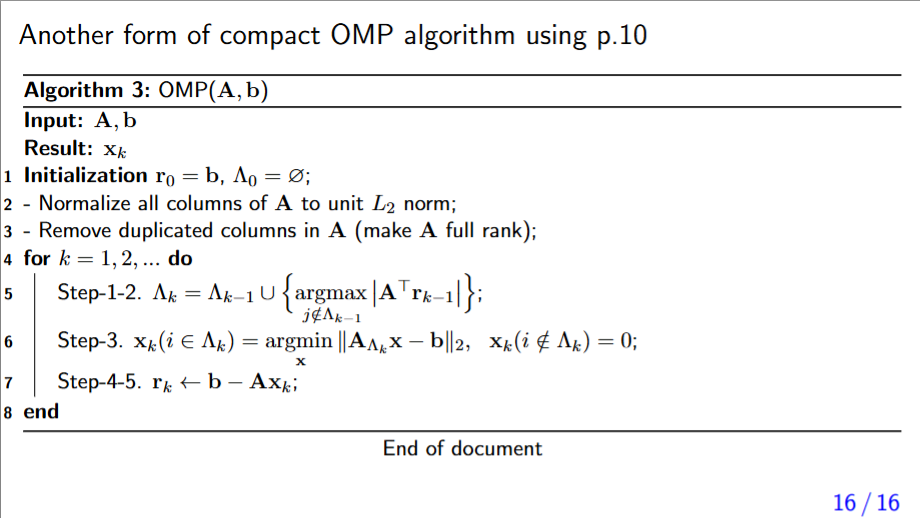
\includegraphics[width=0.8\linewidth,height=\textheight,keepaspectratio]{C:/Users/NinjaBoyASUS/OneDrive/Dokumen/Abhi/Internship/OMP-Python/omp_algorithm.png}

}

\caption{OMP Algorithm}

\end{figure}%

This algorithm can be implemented in MATLAB and Python with necessary
toolboxes and libraries.

\subsection{3.1.1 Algorithm
Implementation}\label{algorithm-implementation}

\begin{itemize}
\tightlist
\item
  \textbf{MATLAB}
\end{itemize}

Here, the sum of two sinusoids is taken as input and it is made sparse
using the built-in dft matrix taken as the basis (\(\Psi\)) and is
measured using a random gaussian matrix (\(\Phi\)).

The algorithm was initially tested directly in frequncy domain. In its
ideal form(ie. without noise), for a low enough sparsity, the algorithm
perfectly reconstructed the frequency and the amplitude values of
compressed signal. Then, two values of noise was given(SNR=0dB and
SNR=20dB). The Algorithm was able to reconstruct the signal
near-perfectly for an SNR of 20 dB. For an SNR of 0 dB(signal
power=noise power), the results were more inaccurate, both in terms of
position on the graph(frequency) and the amplitude values. Still, the
algorithm was able to reconstruct some parts of the signal with a fair
amount of accuracy.

\begin{figure}[H]

{\centering \includegraphics[width=0.8\linewidth,height=\textheight,keepaspectratio]{C:/Users/NinjaBoyASUS/Downloads/omp-matlab-sin-fig.png}

}

\caption{OMP Signal Reconstruction:Ideal (No noise added)}

\end{figure}%

\begin{figure}[H]

{\centering \includegraphics[width=0.8\linewidth,height=\textheight,keepaspectratio]{C:/Users/NinjaBoyASUS/Downloads/omp-matlab-sin-fig.png}

}

\caption{OMP Signal Reconstruction: 20dB}

\end{figure}%

\begin{figure}[H]

{\centering \includegraphics[width=0.8\linewidth,height=\textheight,keepaspectratio]{C:/Users/NinjaBoyASUS/Downloads/omp-matlab-sin-fig.png}

}

\caption{OMP Signal Reconstruction: 0dB}

\end{figure}%

Next, the code was used to implement sinusoids in time domain. A real
sum of 5 sinusoids was given as input to the algorithm. Then the output
is plotted along with the original signal to compare them. The algorithm
was able to reconstruct the signal fairly accurately. Smaller peaks of
the input signal was harder to reconstruct for the algorithm, and also,
there was a reduction in the amplitude of the reconstructed signal w.r.t
the original signal.A slight phase shift was observed in some outputs
when the code is run for different random inputs.

\begin{figure}[H]

{\centering \includegraphics[width=0.8\linewidth,height=\textheight,keepaspectratio]{C:/Users/NinjaBoyASUS/Downloads/omp-matlab-sin-fig.png}

}

\caption{OMP Signal Reconstruction: sinusoidal input}

\end{figure}%

\begin{itemize}
\item
  \textbf{Python}

  Libraries like \textbf{numpy} and \textbf{matplotlib} are imported for
  mathematical operations and plotting results respectively.

  \begin{itemize}
  \item
    \textbf{Stage 1:} The basic implementation was done by taking length
    of signal (n), number of measurements (m) and non-zero values or
    sparsity (k) as input. The sensing matrix was assumed to be filled
    with random gaussian values.
  \item
    \textbf{Stage 2:} The next stage involved taking a sum of three
    sinusoidal signals as input signal (k = 3) and it is converted to a
    more sparser domain with \textbf{Discrete Cosine Transform (DCT)}.
    The function is used by importing the \textbf{scipy} library. While
    initially k was fixed, it is then taken as an input from user. DCT
    was initially tested for a single sine wave as well as for sum of
    sine waves of different frequencies, as shown in the figure below.
  \item
    \textbf{Stage 3:} In the above stages, reconstruction was observed
    for pure signals. So, a noise (in dB) was introduced before the
    reconstruction process.
  \end{itemize}
\end{itemize}

All these stages were plotted and the error was calculated and observed.

\subsection{3.1.2 Monte-Carlo Trials}\label{monte-carlo-trials}

Monte Carlo trials are a broad class of computational algorithms that
rely on repeated random sampling to obtain numerical results. The is
used to understand the behaviour of the algorithm under change in
parameters, including sparsity, noise and number of measurements taken.
It is useful for analysis, understanding its performance for various
values of multiple inputs. In other words, this acts like a testbench
for the algorithm.

The input values were stored in a list and these were fed to the trial
algorithm. The error was calculated for a number of trials for the same
input values, and only the average error is plotted to prevent unwanted
variations in reconstruction.

\subsection{3.1.3 Observations \& Results}\label{observations-results}

For \textbf{Stage 1} implementation, the sparse matrix is already
created by specifying k. So, the compressed matrix (y) is generated by
just multiplying sensing matrix (\(\Theta\)) and the generated sparse
matrix (s). The results are plotted as shown below,

\begin{figure}[H]

{\centering 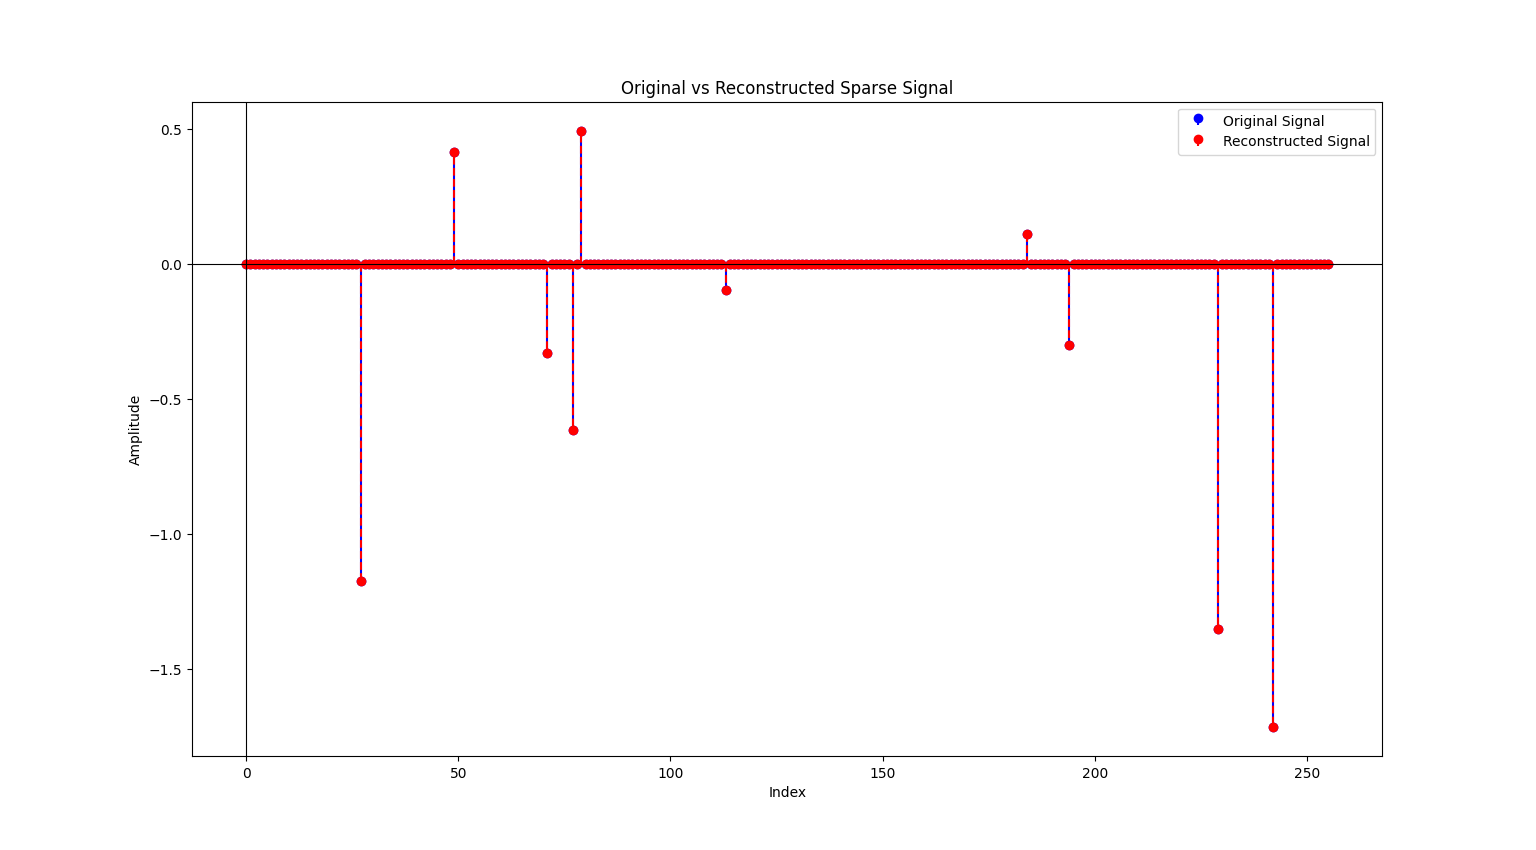
\includegraphics[width=0.8\linewidth,height=\textheight,keepaspectratio]{D:/Dokumen/Abhi/Internship/OMP-Python/omp-gaussian/True-Recon/omp-alg-op1.png}

}

\caption{OMP Algorithm Stage 1 Implementation: Perfect Reconstruction}

\end{figure}%

While the reconstruction as shown above is very accurate, it is not
always the case. As sparsity increases, the measurements to be taken
also increases. Hence, there are some necessary conditions for perfect
recovery of a signal. As mentioned in \autocite{rani-cs}, the relation
between n, m and k is:-

\begin{equation}
\boxed{
    m \geq C \cdot k \cdot \log\left(\frac{n}{k}\right)
}
\end{equation}

where \textbf{C} is a constant almost equal to 2.

Hence, if the above equation is not satisfied, then reconstruction is
very difficult. The failed reconstruction is shown below.

\begin{figure}[H]

{\centering 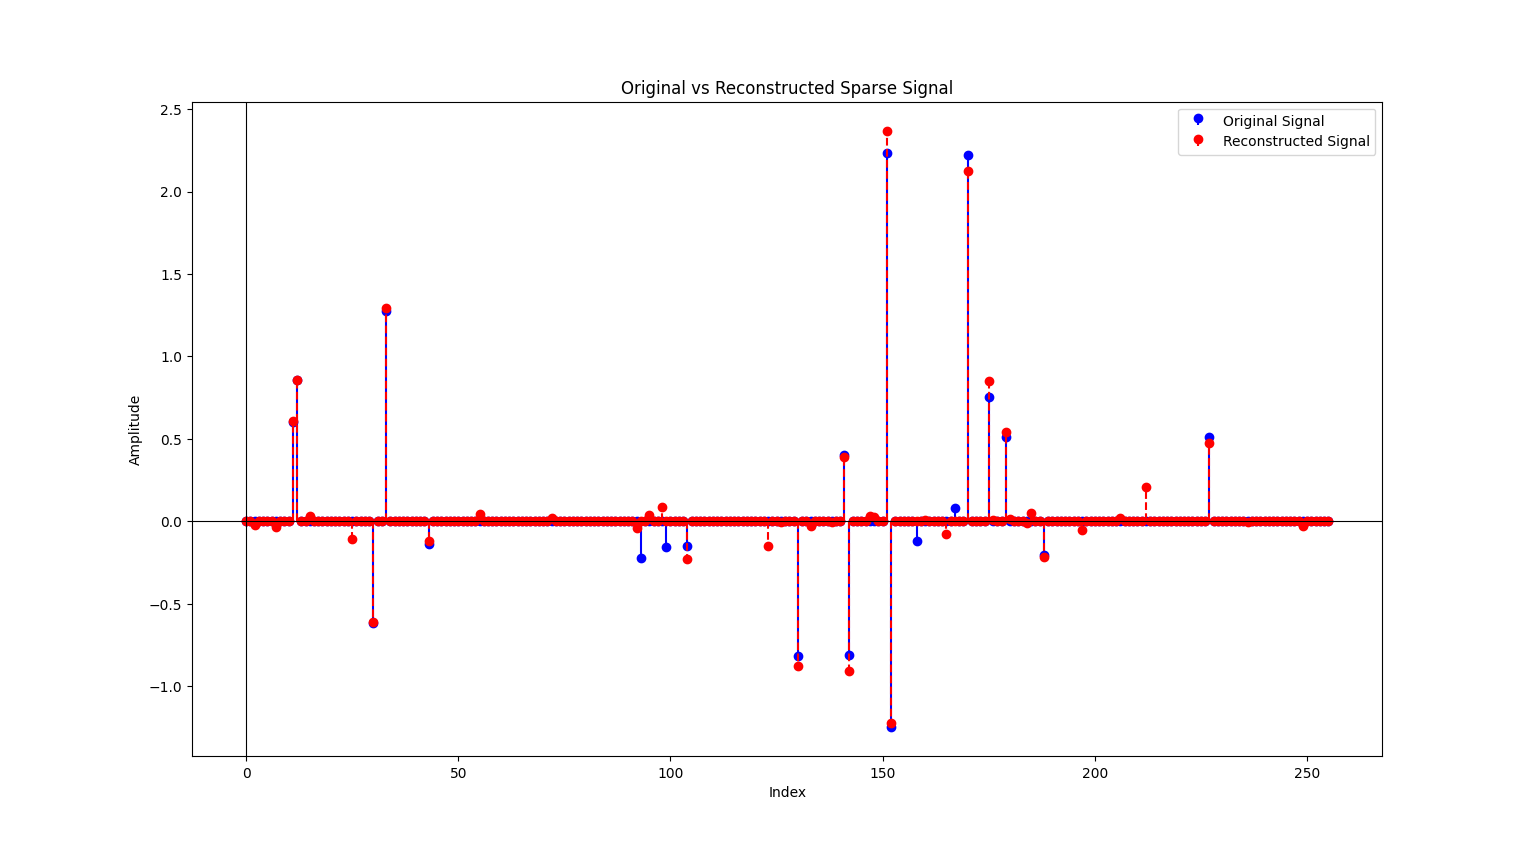
\includegraphics[width=0.8\linewidth,height=\textheight,keepaspectratio]{D:/Dokumen/Abhi/Internship/OMP-Python/omp-gaussian/Error/omp-alg-op2.png}

}

\caption{OMP Algorithm Stage 1 Implementation: Failed Reconstruction}

\end{figure}%

When it comes to \textbf{Stage 2} implementation, the sensing matrix is
divided into a basis matrix and measurement matrix. The basis matrix is
used to convert our input signal to a sparser signal. For sinusoidal
inputs, it is best to represent the signals in its frequency domain. So,
FFT or DCT can be used. Since, all sinusoids are real signals, DCT was
possible. The sum of sinusoids were converted to DCT and the results are
being plotted to check its sparsity.

\begin{figure}[H]

{\centering 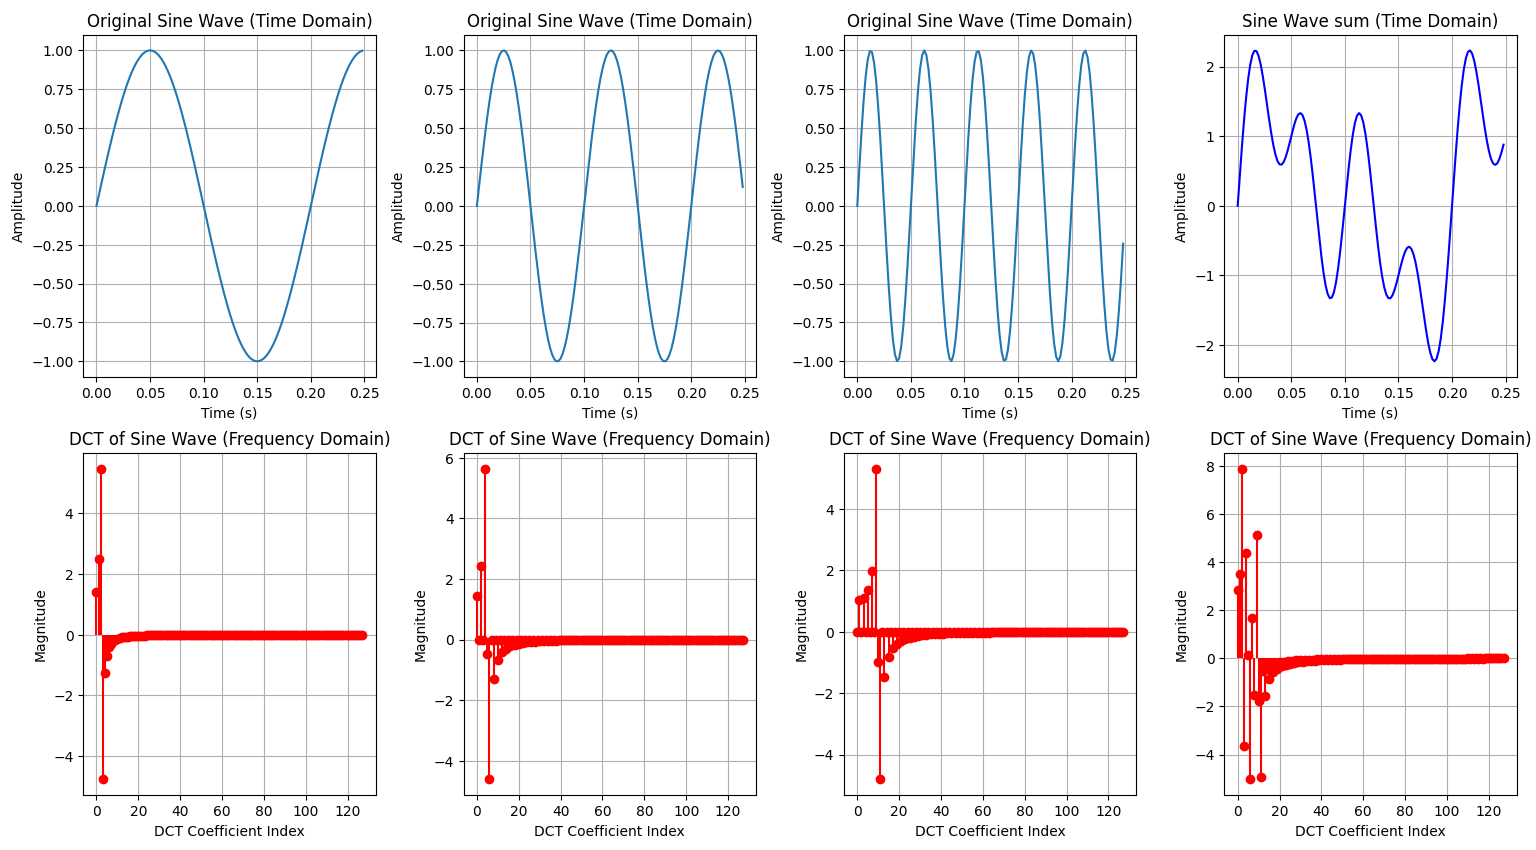
\includegraphics[width=0.8\linewidth,height=\textheight,keepaspectratio]{D:/Dokumen/Abhi/Internship/OMP-Python/omp-sin/sine-dct.png}

}

\caption{OMP Algorithm Stage 2 Implementation: DCT Basis on Sinusoidal
signals}

\end{figure}%

The sinusoidal signal is initially tested for various values of n and m,
keeping k = 3. Some of the results are plotted as shown,

\begin{figure}[H]

{\centering 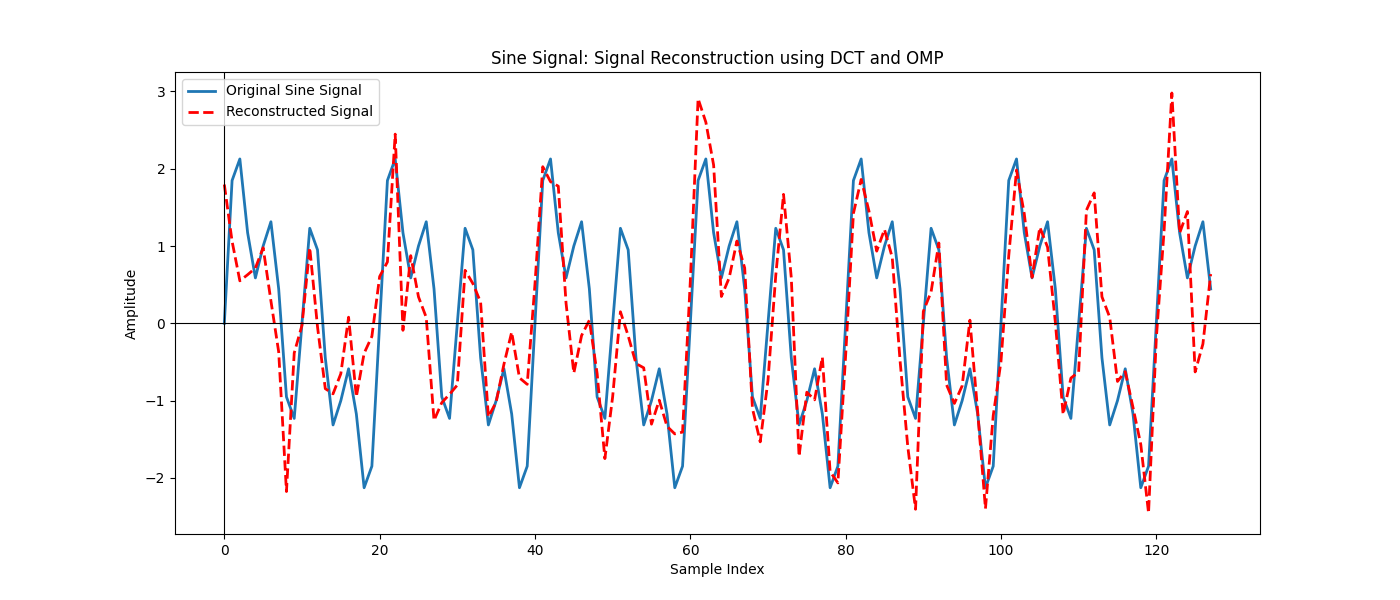
\includegraphics[width=0.8\linewidth,height=\textheight,keepaspectratio]{D:/Dokumen/Abhi/Internship/OMP-Python/omp-sin/omp-sine-n128-m60.png}

}

\caption{OMP Algorithm Stage 2 Implementation: For n = 128, m = 60}

\end{figure}%

\begin{figure}[H]

{\centering 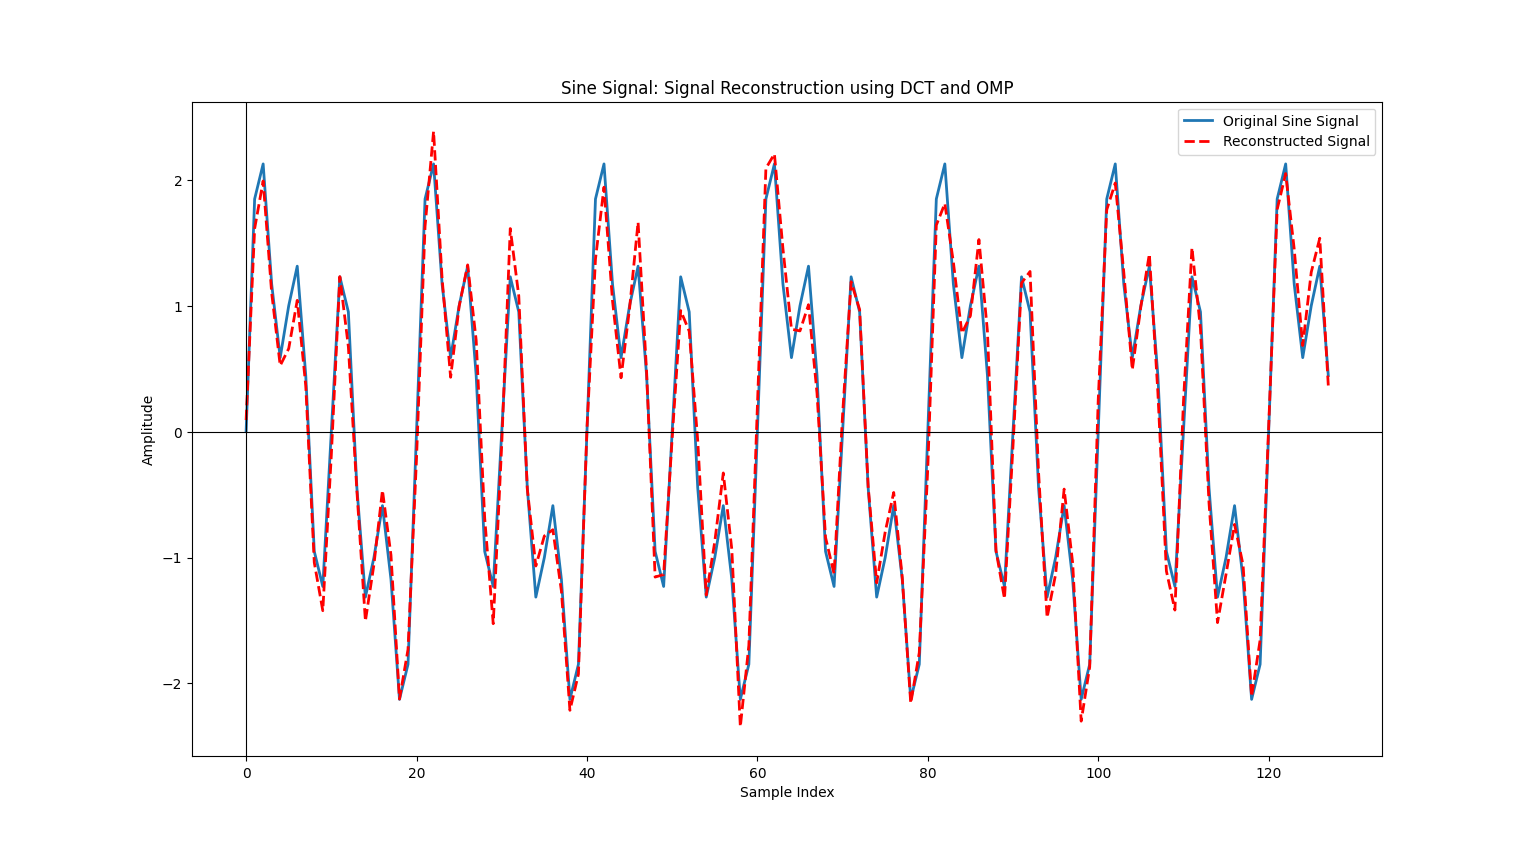
\includegraphics[width=0.8\linewidth,height=\textheight,keepaspectratio]{D:/Dokumen/Abhi/Internship/OMP-Python/omp-sin/omp-sine-n128-m100.png}

}

\caption{OMP Algorithm Stage 2 Implementation: For n = 128, m = 100}

\end{figure}%

So, generally we can say as \textbf{number of measurements increases,
the reconstruction error decreases}. Till now, no noise has been
considered during the reconstruction. To analyse the algorithm for each
value of n, m, k and even noise, it is difficult for us to understand
the trend of error. So, a Monte Carlo trial has been implemented on the
OMP algorithm for three variable parameters, \textbf{measurements},
\textbf{sparsity} and \textbf{noise}. So, all three parameters are
compared and the results are plotted.

\begin{figure}[H]

{\centering 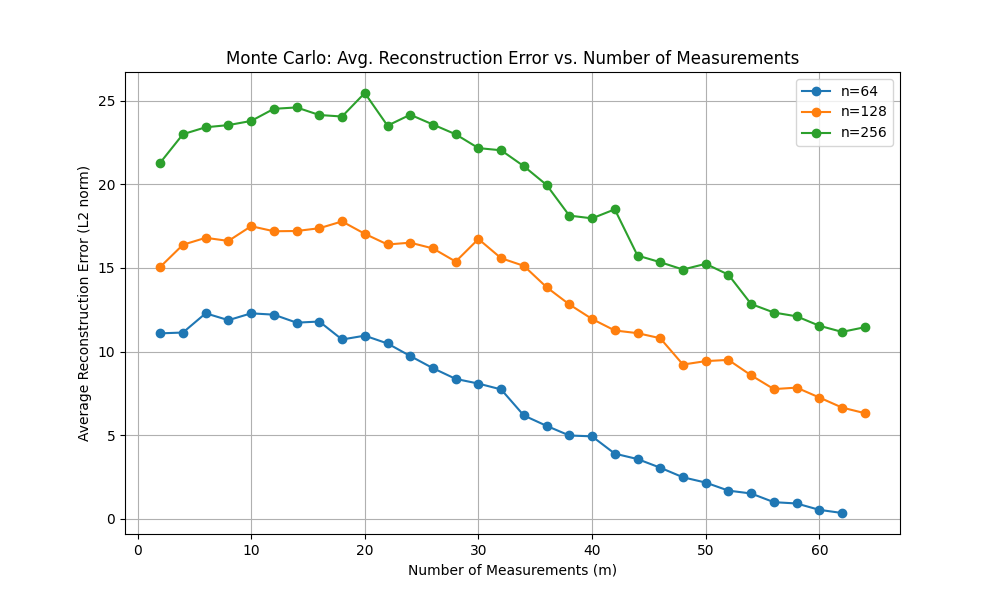
\includegraphics[width=0.8\linewidth,height=\textheight,keepaspectratio]{D:/Dokumen/Abhi/Internship/OMP-Python/omp-sin/omp-montecarlo.png}

}

\caption{Monte Carlo Trial: Measurements (m)}

\end{figure}%

The analysis above is for noiseless, fixed sparsity (k = 3)
reconstruction.

\begin{figure}[H]

{\centering 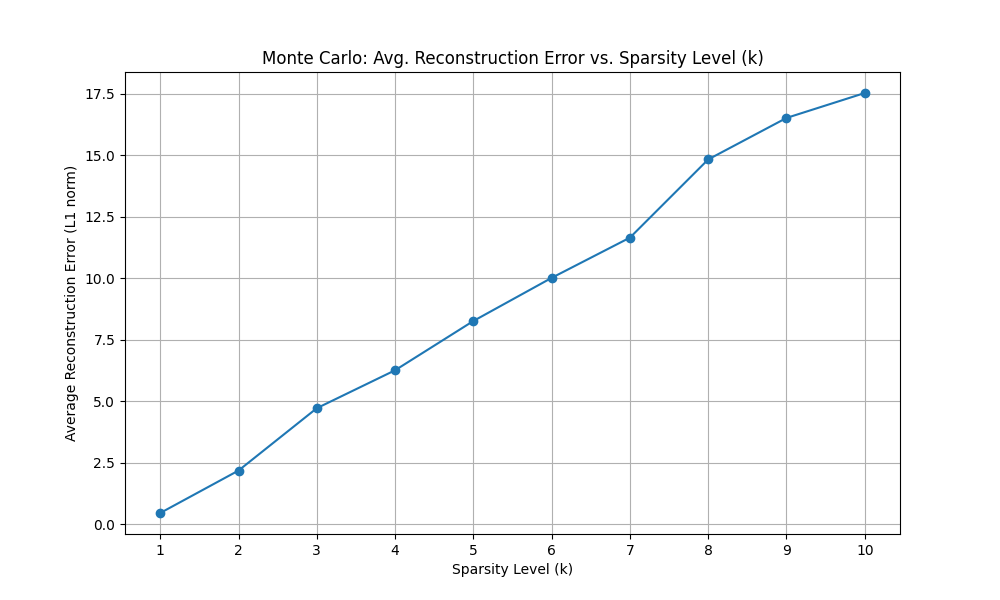
\includegraphics[width=0.8\linewidth,height=\textheight,keepaspectratio]{D:/Dokumen/Abhi/Internship/OMP-Python/omp-sin/omp-montecarlo-sparsity.png}

}

\caption{Monte Carlo Trial: Sparsity (k)}

\end{figure}%

\begin{figure}[H]

{\centering 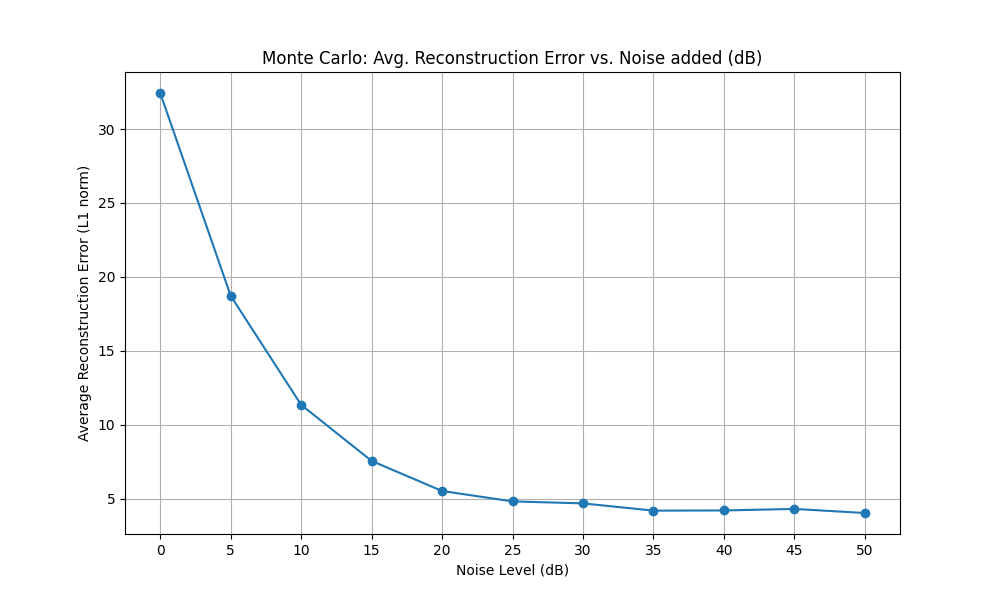
\includegraphics[width=0.8\linewidth,height=\textheight,keepaspectratio]{D:/Dokumen/Abhi/Internship/OMP-Python/omp-sin/omp-montecarlo-noise.png}

}

\caption{Monte Carlo Trial: Noise (in dB)}

\end{figure}%

Conclusion needed\ldots\ldots{}

\subsection{3.2 ITERATIVE SHRINKAGE THRESHOLDING ALGORITHM
(ISTA)}\label{iterative-shrinkage-thresholding-algorithm-ista}

The ISTA is an iterative, convex optimisation method for solving sparse
signal recovery problems, particularly those formulated as LASSO or
basis pursuit denoising. ISTA iteratively updates the solution by
applying a gradient descent step followed by a soft-thresholding
(shrinkage) operation to promote sparsity. The general steps are:

\begin{enumerate}
\def\labelenumi{\arabic{enumi}.}
\tightlist
\item
  Initialize the sparse coefficient vector.
\item
  At each iteration, perform a gradient descent step to minimize the
  data fidelity term.
\item
  Apply the soft-thresholding operator to enforce sparsity.
\item
  Repeat until convergence.
\end{enumerate}

These steps are as shown, from \autocite{fast-sparse-coding}

\begin{figure}[H]

{\centering 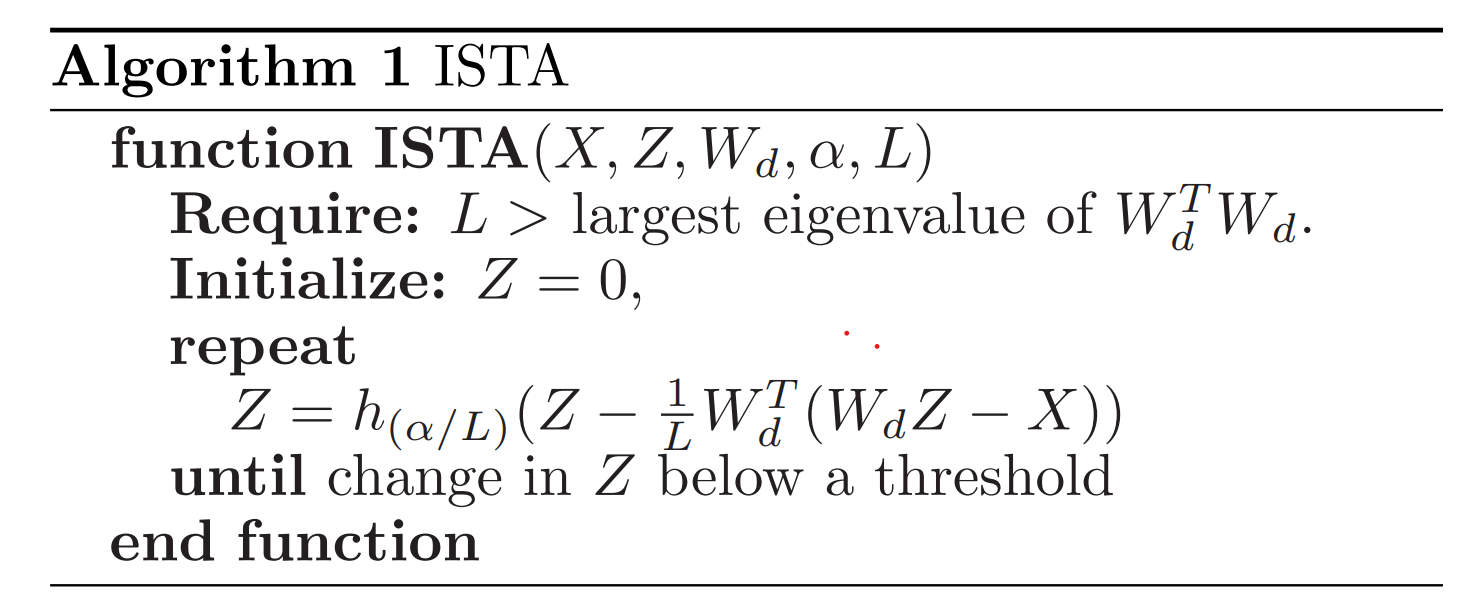
\includegraphics[width=0.8\linewidth,height=\textheight,keepaspectratio]{D:/Dokumen/Abhi/Internship/ISTA-Python/img/ista-alg.png}

}

\caption{ISTA Algorithm}

\end{figure}%

\subsubsection{3.2.1 Algorithm Implementation \& Monte Carlo
Trial}\label{algorithm-implementation-monte-carlo-trial}

Just like in OMP implemntation, the basic libraries were imported and
the sinusoidal input is converted to its sparser domain using DCT. The
soft thresholding function plays a role in enforcing sparsity by
shrinking very small values to zero. Since convergence is very slow in
ISTA, the number of iterations are higher than that of OMP.

Monte Carlo has been implemented in a very similar manner as that of OMP
and it has been checked for all the 3 paramters. Moreover, both the
algorithms have been compared for these parameters, and their
performance has been observed and analysed.

\subsubsection{3.2.2 Observations \&
Results}\label{observations-results-1}

Implementing ISTA for a sinusoidal input had some similarities with that
of the OMP algorithm. The trends in the major 3 parameters are same for
both the algorithms. Initially ISTA was checked for pure reconstruction,
that is no noise interfernce. The result is as plotted,

\begin{figure}[H]

{\centering 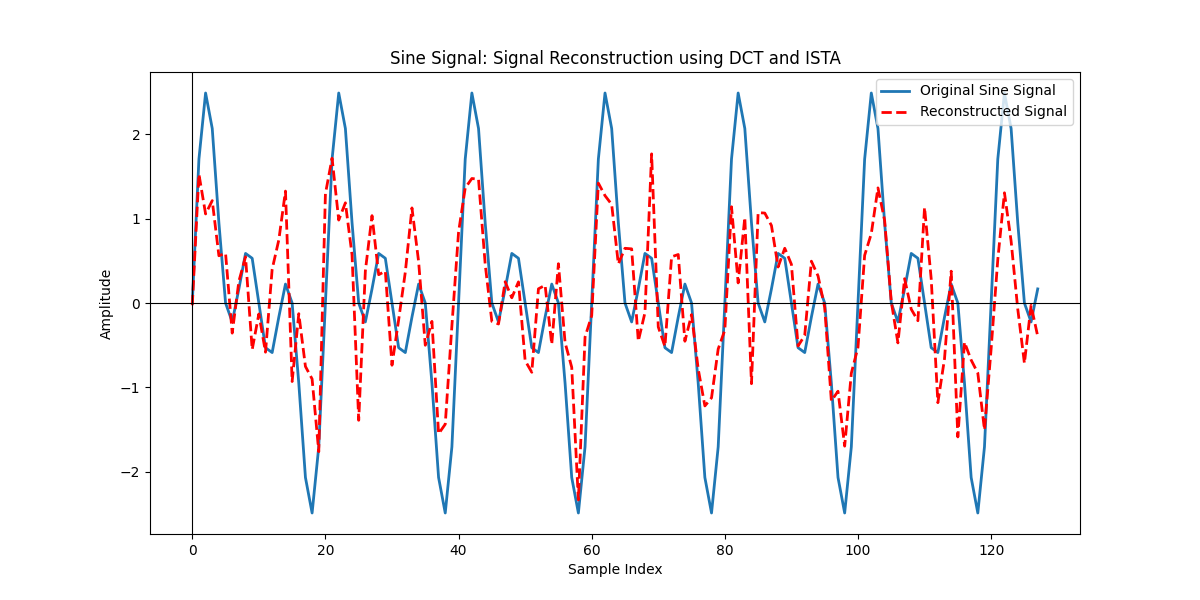
\includegraphics[width=0.8\linewidth,height=\textheight,keepaspectratio]{D:/Dokumen/Abhi/Internship/ISTA-Python/img/istaa-sin-dct.png}

}

\caption{ISTA Algorithm Implementation (Ideal)}

\end{figure}%

It is observed that as the number of iterations for ISTA increases, the
error decreases.

Now, when noise is added during the process, its performance is also as
shown,

\begin{figure}[H]

{\centering 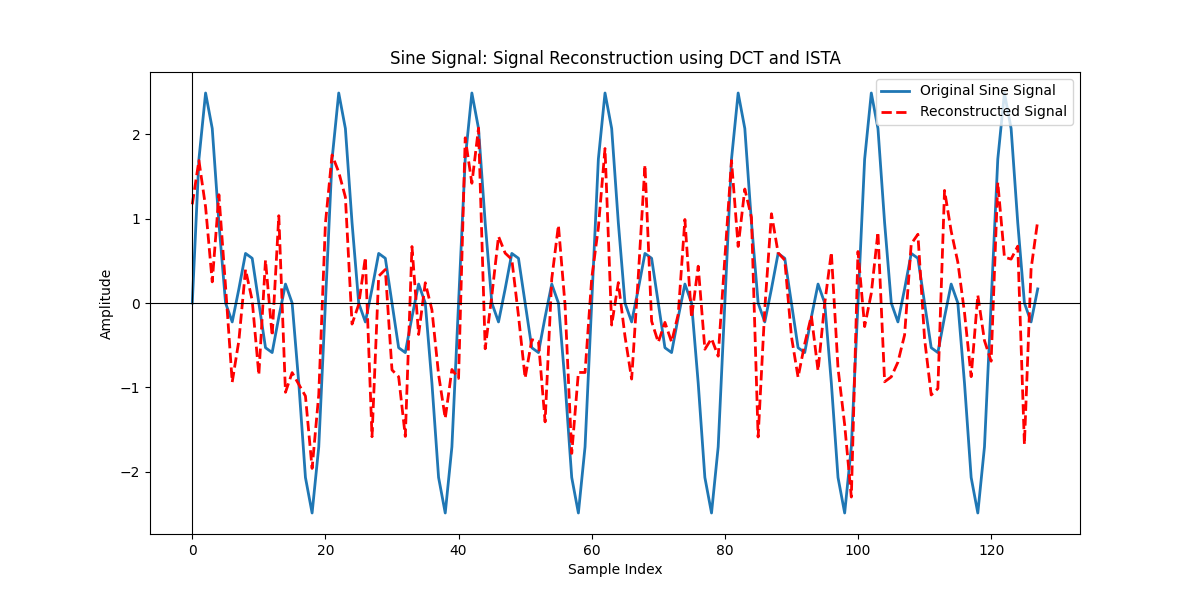
\includegraphics[width=0.8\linewidth,height=\textheight,keepaspectratio]{D:/Dokumen/Abhi/Internship/ISTA-Python/img/istaa-sin-dct-noise.png}

}

\caption{ISTA Algorithm Implementation (With Noise)}

\end{figure}%

Here, unlike OMP, ISTA is very resistant to noise variation and hence
explains its advantage over OMP. That is because of the shrinkage
function, which shrinks small coefficients to zero and its
regularisation term penalises the high variance solutions. In contrary,
OMP being a greedy algorithm, tends to select the noisy atoms causing to
succumb to the effect of noise. Hence, ISTA is more robust to noise than
OMP.

The Monte Carlo for ISTA has been implemented with varying measurements
for every value of n.~The results are to some extent similar to that of
the OMP, that is the reconstruction error follows an inverse
relationship with the number of measurements, which is as shown below,

\begin{figure}[H]

{\centering 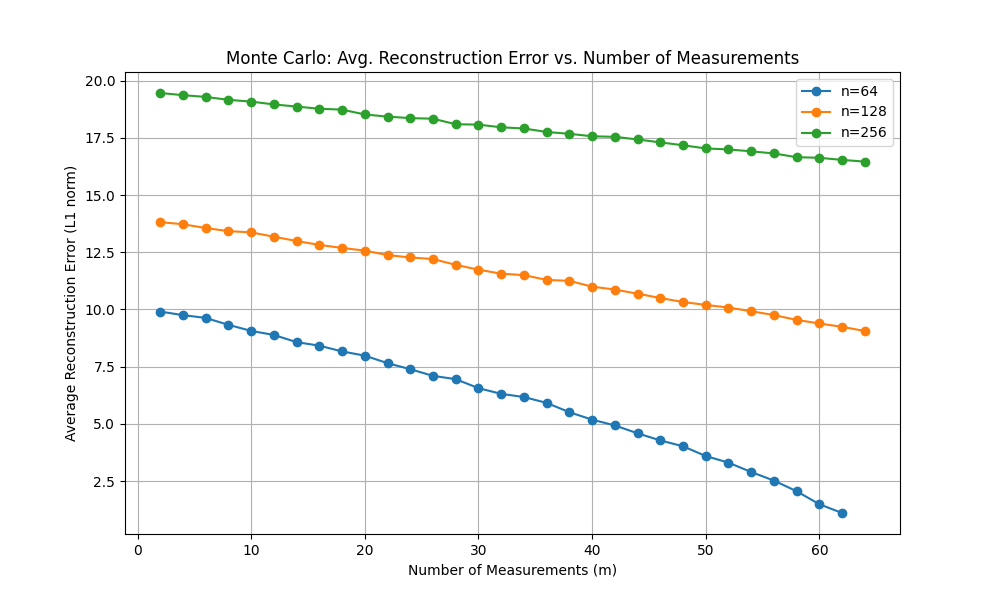
\includegraphics[width=0.8\linewidth,height=\textheight,keepaspectratio]{D:/Dokumen/Abhi/Internship/ISTA-Python/img/istaa-montecarlo.png}

}

\caption{Monte Carlo Trial: Measurements (m)}

\end{figure}%

With these 3 parameters used for the trial, it can be done to compare
both ISTA and OMP. This is done so as to assess and understand the scope
of the algorithm for future work, etc. The comparisons are shown below

\begin{figure}[H]

{\centering 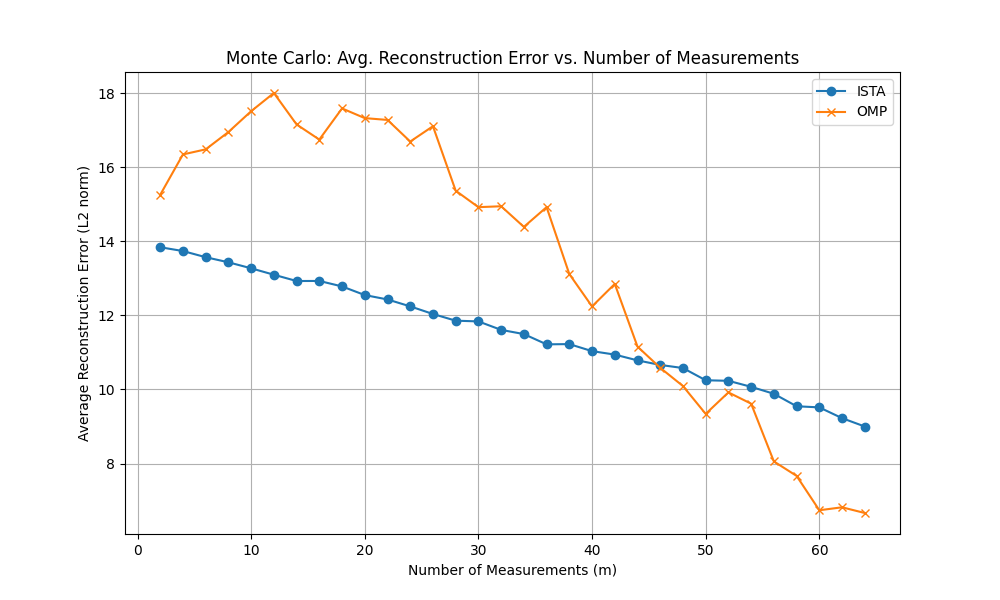
\includegraphics[width=0.8\linewidth,height=\textheight,keepaspectratio]{D:/Dokumen/Abhi/Internship/Comparison/montecarlo-omp-ista-measurements.png}

}

\caption{OMP v/s ISTA (m)}

\end{figure}%

\begin{figure}[H]

{\centering 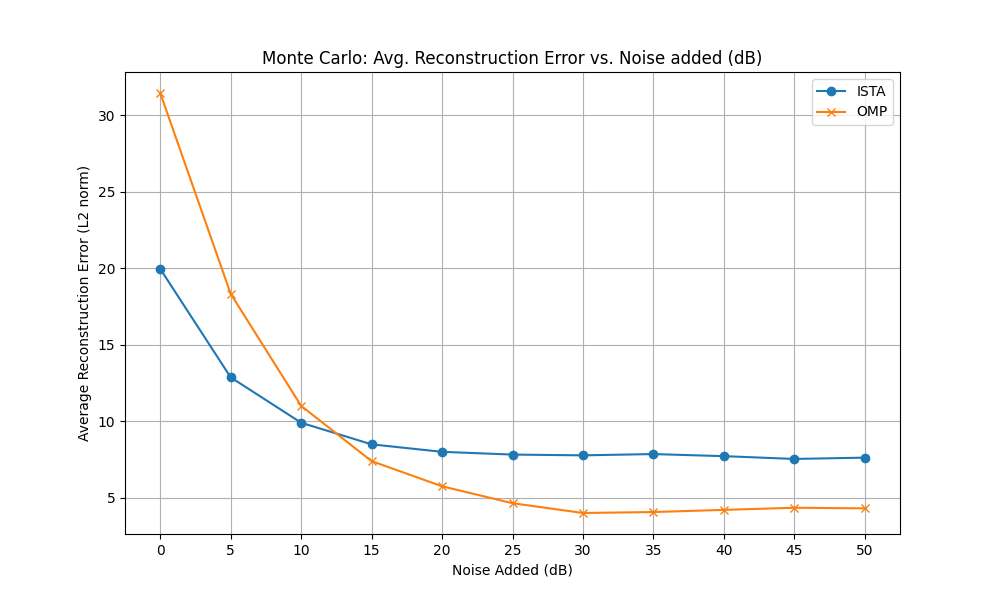
\includegraphics[width=0.8\linewidth,height=\textheight,keepaspectratio]{D:/Dokumen/Abhi/Internship/Comparison/montecarlo-omp-ista-noise.png}

}

\caption{OMP v/s ISTA (noise)}

\end{figure}%

\begin{figure}[H]

{\centering 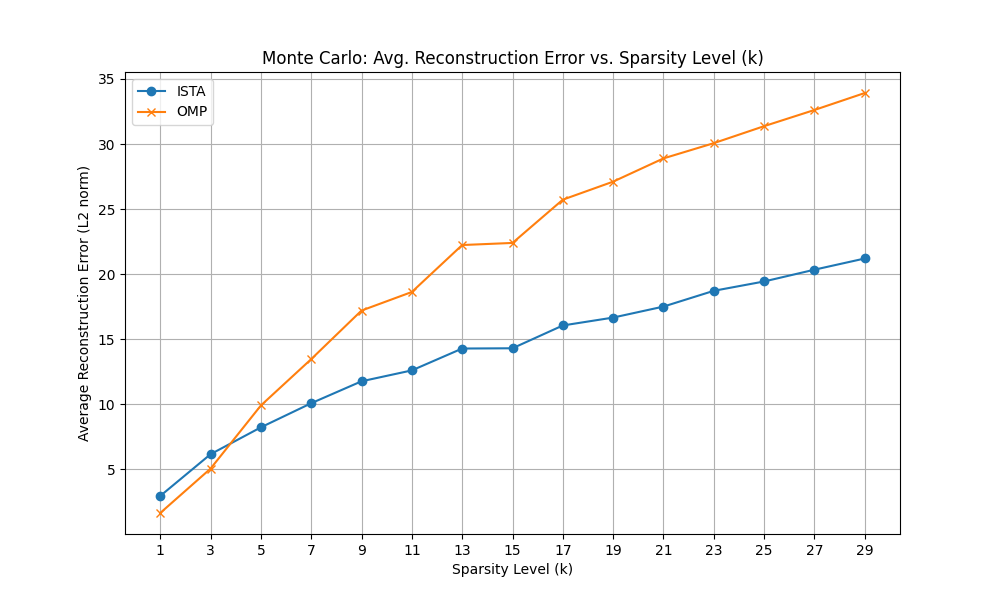
\includegraphics[width=0.8\linewidth,height=\textheight,keepaspectratio]{D:/Dokumen/Abhi/Internship/Comparison/montecarlo-omp-ista-sparsity.png}

}

\caption{OMP v/s ISTA (sparsity)}

\end{figure}%

In summary, both OMP and ISTA have their own strengths and are suitable
for different scenarios in compressed sensing-based radar signal
processing:

\begin{itemize}
\item
  \textbf{OMP} excels when the signal is highly sparse and the number of
  measurements is sufficient. It is computationally efficient and
  provides accurate reconstruction in low-noise environments. However,
  its performance degrades with increased noise or when the sparsity
  assumption is violated.
\item
  \textbf{ISTA} is more robust to noise due to its regularization and
  shrinkage steps. It can handle less sparse signals and noisy
  measurements better than OMP, albeit at the cost of slower convergence
  and higher computational complexity. It is best in handling
  undersampled and noisy data.
\end{itemize}

The choice between OMP and ISTA depends on the specific requirements of
the application, such as the expected sparsity of the signal, noise
levels, and computational resources. In practice, a trade-off must be
made between reconstruction accuracy, noise robustness, and
computational efficiency.

\subsection{3.3 COORDINATE DESCENT (CoD)}\label{coordinate-descent-cod}

Coordinate Descent is a simple yet powerful optimization algorithm that
is widely used in compressed sensing applications, especially for
solving large-scale sparse recovery problems such as LASSO (Least
Absolute Shrinkage and Selection Operator). It works by minimizing (or
maximizing) a function by solving for one variable at a time while
keeping the others fixed. The process repeats, cycling through each
variable (or ``coordinate'') in turn, updating its value to reduce the
objective function. The general steps are: 1. Initialize the sparse
coefficient vector. 2. For each coordinate (variable), update its value
by minimizing the objective function with respect to that coordinate,
keeping all other variables fixed. 3. Apply the soft-thresholding
operator to the updated coordinate to enforce sparsity. 4. Repeat steps
2 and 3 for all coordinates, cycling through them until convergence.

\begin{center}
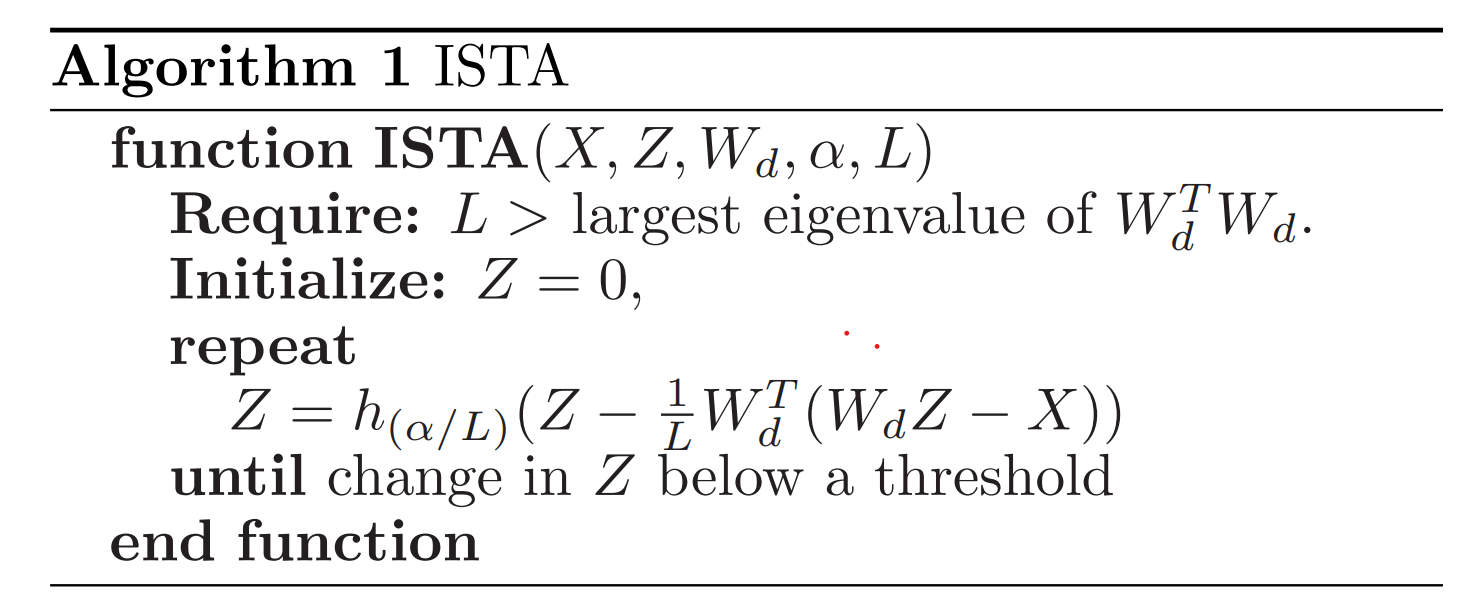
\includegraphics[width=0.8\linewidth,height=\textheight,keepaspectratio]{D:/Dokumen/Abhi/Internship/ISTA-Python/img/ista-alg.png}
\end{center}

\subsubsection{3.3.1 Algorithm
Implementation}\label{algorithm-implementation-1}

In the MATLAB implementation of CoD algorithm, The process begins by
generating a sparse signal (z\_true) and its measurement (y) using a
random sensing matrix (Phi). The main loop iteratively updates each
coordinate of the sparse coefficient vector (z) by applying the
soft-thresholding operator, which enforces sparsity. At each iteration,
the coordinate with the largest change is selected and updated to
minimize the objective function. The reconstructed signal is then
compared to the original, and the mean squared error (MSE) is tracked
over iterations to monitor convergence. The code concludes by plotting
both the original and reconstructed signals, as well as the MSE
progression, illustrating the effectiveness of the CoD algorithm in
recovering sparse signals.

\subsubsection{3.3.2 Observations \&
Results}\label{observations-results-2}

Two types of implementations were considered- an ideal noiseless input
signal and an input signal with 10dB of noise. For the ideal condition,
multple values of m were considered(32,64 and 128) for n = 128 and the
original vs reconstructed signal graphs were plotted.

\begin{figure}[H]

{\centering \includegraphics[width=0.8\linewidth,height=\textheight,keepaspectratio]{abar-cs_files/mediabag/cod_m32.png}

}

\caption{CoD Algorithm}

\end{figure}%

\begin{figure}[H]

{\centering \includegraphics[width=0.8\linewidth,height=\textheight,keepaspectratio]{abar-cs_files/mediabag/cod_m64.png}

}

\caption{CoD Algorithm}

\end{figure}%

\begin{figure}[H]

{\centering \includegraphics[width=0.8\linewidth,height=\textheight,keepaspectratio]{abar-cs_files/mediabag/cod_m128.png}

}

\caption{CoD Algorithm}

\end{figure}%

Also, the plot between the Mean Squared Error(MSE) and the number of
iterations gives us the convergence of the algorithm.

\begin{figure}[H]

{\centering 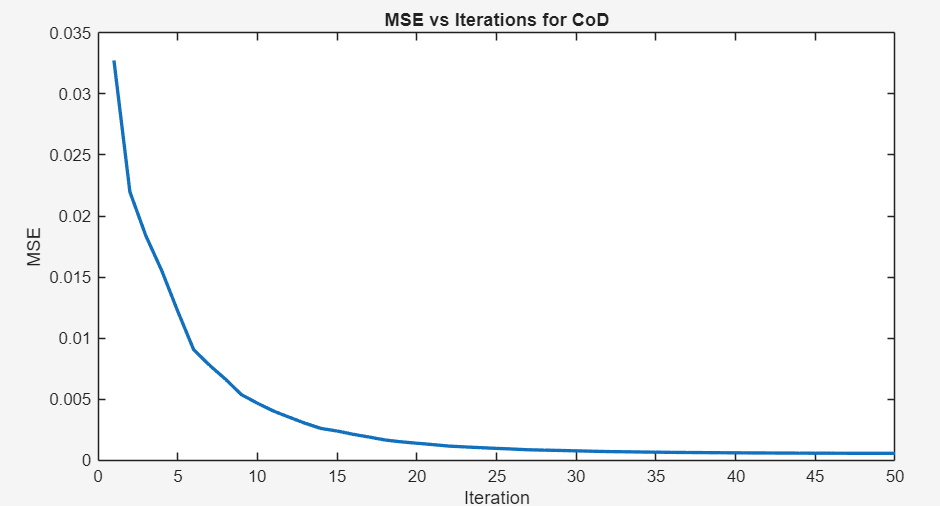
\includegraphics[width=0.8\linewidth,height=\textheight,keepaspectratio]{abar-cs_files/mediabag/cod_conv_ideal.png}

}

\caption{CoD Algorithm}

\end{figure}%

Now, for the noisy implementation m = 32 and 64 were considered for n =
128 and the corresponding graphs were plotted. For m = 32, the original
vs reconstructed signal graph:

\begin{figure}[H]

{\centering 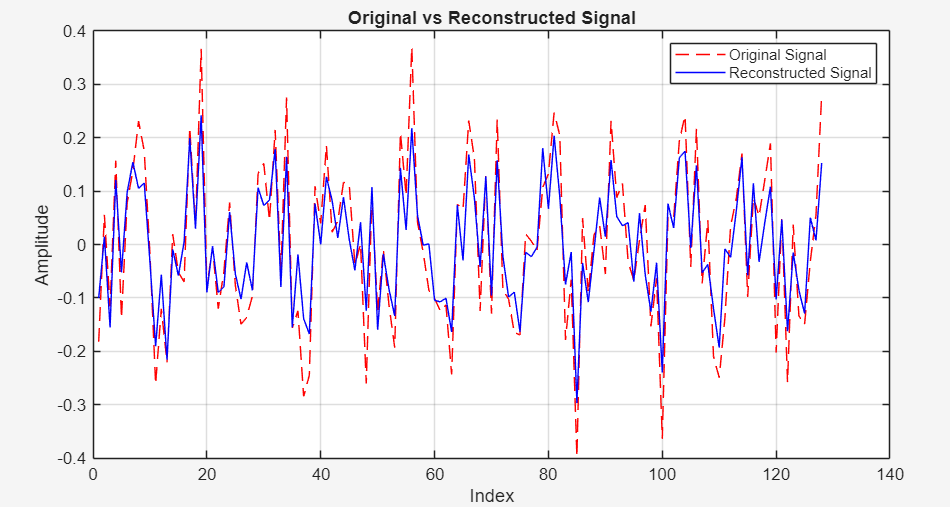
\includegraphics[width=0.8\linewidth,height=\textheight,keepaspectratio]{abar-cs_files/mediabag/cod_m32_noisy1.png}

}

\caption{CoD Algorithm}

\end{figure}%

The Iterations vs MSE graph for m = 32:

\begin{figure}[H]

{\centering \includegraphics[width=0.8\linewidth,height=\textheight,keepaspectratio]{abar-cs_files/mediabag/cod_m32_noisy_mse.png}

}

\caption{CoD Algorithm}

\end{figure}%

For m = 64, the original vs reconstructed signal graph:

\begin{figure}[H]

{\centering \includegraphics[width=0.8\linewidth,height=\textheight,keepaspectratio]{abar-cs_files/mediabag/cod_m64_noisy1.png}

}

\caption{CoD Algorithm}

\end{figure}%

The Iterations vs MSE graph for m = 64:

\begin{figure}[H]

{\centering 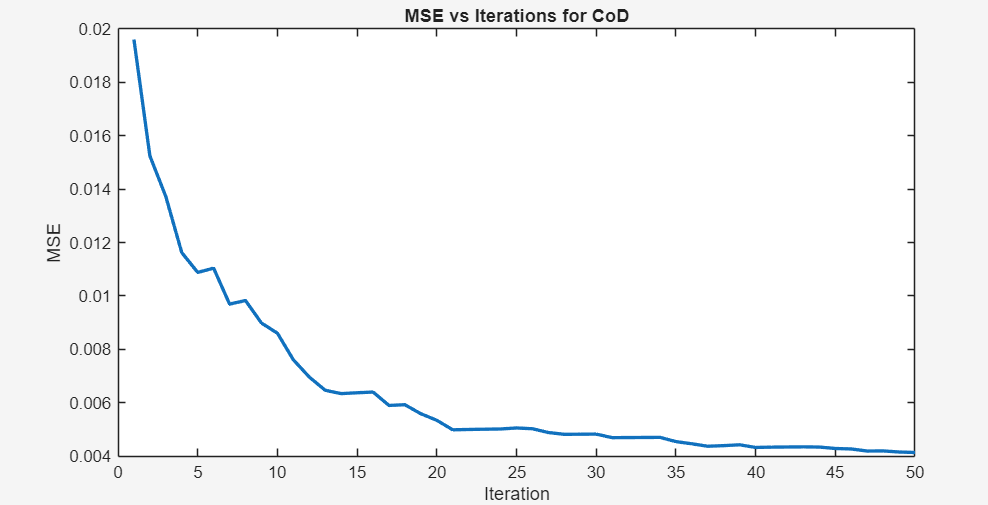
\includegraphics[width=0.8\linewidth,height=\textheight,keepaspectratio]{abar-cs_files/mediabag/cod_m64_noisy_mse.png}

}

\caption{CoD Algorithm}

\end{figure}%

\newpage

\mainsection{CHAPTER 4: RADAR APPLICATIONS}

\newpage

\mainsection{CHAPTER 5: FUTURE SCOPE}

\emph{Summary and conclusion go here\ldots{}} \newpage

\mainsection{REFERENCES}

\section{References}\label{references}

\printbibliography[heading=none]

\newpage

\mainsection{APPENDICES}

\textbf{CODE:-} - \textbf{OMP Implementation (Python)}

\begin{Shaded}
\begin{Highlighting}[]
\ImportTok{import}\NormalTok{ numpy }\ImportTok{as}\NormalTok{ np}
\ImportTok{import}\NormalTok{ matplotlib.pyplot }\ImportTok{as}\NormalTok{ plt}
\ImportTok{from}\NormalTok{ scipy.fftpack }\ImportTok{import}\NormalTok{ dct, idct}
\ImportTok{from}\NormalTok{ numpy.linalg }\ImportTok{import}\NormalTok{ norm}

\KeywordTok{def}\NormalTok{ generate\_sine\_signal(n, k, freq}\OperatorTok{=}\DecValTok{5}\NormalTok{, fs}\OperatorTok{=}\DecValTok{100}\NormalTok{):}
\NormalTok{    t }\OperatorTok{=}\NormalTok{ np.arange(n) }\OperatorTok{/}\NormalTok{ fs}
\NormalTok{    sum\_signal }\OperatorTok{=}\NormalTok{ np.zeros(n)}
    \ControlFlowTok{for}\NormalTok{ i }\KeywordTok{in} \BuiltInTok{range}\NormalTok{(}\DecValTok{1}\NormalTok{, k }\OperatorTok{+} \DecValTok{1}\NormalTok{):}
\NormalTok{        freq }\OperatorTok{=}\NormalTok{ i }\OperatorTok{*} \DecValTok{5}
\NormalTok{        sum\_signal }\OperatorTok{+=}\NormalTok{ np.sin(}\DecValTok{2} \OperatorTok{*}\NormalTok{ np.pi }\OperatorTok{*}\NormalTok{ freq }\OperatorTok{*}\NormalTok{ t)}
    \ControlFlowTok{return}\NormalTok{ sum\_signal}

\KeywordTok{def}\NormalTok{ measurement(m, n):}
\NormalTok{    Psi }\OperatorTok{=}\NormalTok{ idct(np.eye(n), norm}\OperatorTok{=}\StringTok{\textquotesingle{}ortho\textquotesingle{}}\NormalTok{)}
\NormalTok{    Phi }\OperatorTok{=}\NormalTok{ np.random.randn(m, n)}
    \ControlFlowTok{return}\NormalTok{ Phi }\OperatorTok{@}\NormalTok{ Psi}

\KeywordTok{def}\NormalTok{ omp(y, A, tol}\OperatorTok{=}\FloatTok{1e{-}6}\NormalTok{):}
\NormalTok{    m, n }\OperatorTok{=}\NormalTok{ A.shape}
\NormalTok{    r }\OperatorTok{=}\NormalTok{ y.copy()}
\NormalTok{    idx\_set }\OperatorTok{=}\NormalTok{ []}
\NormalTok{    x\_hat }\OperatorTok{=}\NormalTok{ np.zeros(n)}

    \ControlFlowTok{for}\NormalTok{ \_ }\KeywordTok{in} \BuiltInTok{range}\NormalTok{(m):}
\NormalTok{        correlations }\OperatorTok{=}\NormalTok{ A.T }\OperatorTok{@}\NormalTok{ r}
\NormalTok{        idx }\OperatorTok{=}\NormalTok{ np.argmax(np.}\BuiltInTok{abs}\NormalTok{(correlations))}
\NormalTok{        idx\_set.append(idx)}
\NormalTok{        A\_selected }\OperatorTok{=}\NormalTok{ A[:, idx\_set]}
\NormalTok{        x\_ls, \_, \_, \_ }\OperatorTok{=}\NormalTok{ np.linalg.lstsq(A\_selected, y, rcond}\OperatorTok{=}\VariableTok{None}\NormalTok{)}
\NormalTok{        r }\OperatorTok{=}\NormalTok{ y }\OperatorTok{{-}}\NormalTok{ A\_selected }\OperatorTok{@}\NormalTok{ x\_ls}
        \ControlFlowTok{if}\NormalTok{ np.linalg.norm(r) }\OperatorTok{\textless{}}\NormalTok{ tol:}
            \ControlFlowTok{break}

\NormalTok{    x\_hat[idx\_set] }\OperatorTok{=}\NormalTok{ x\_ls}
    \ControlFlowTok{return}\NormalTok{ x\_hat}

\KeywordTok{def}\NormalTok{ add\_noise(y, snr\_db):}
\NormalTok{    signal\_power }\OperatorTok{=}\NormalTok{ np.mean(np.}\BuiltInTok{abs}\NormalTok{(y)}\OperatorTok{**}\DecValTok{2}\NormalTok{)}
\NormalTok{    snr\_linear }\OperatorTok{=} \DecValTok{10}\OperatorTok{**}\NormalTok{(snr\_db }\OperatorTok{/} \DecValTok{10}\NormalTok{)}
\NormalTok{    noise\_power }\OperatorTok{=}\NormalTok{ signal\_power }\OperatorTok{/}\NormalTok{ snr\_linear}
\NormalTok{    noise }\OperatorTok{=}\NormalTok{ np.sqrt(noise\_power) }\OperatorTok{*}\NormalTok{ np.random.randn(}\OperatorTok{*}\NormalTok{y.shape)}
    \ControlFlowTok{return}\NormalTok{ y }\OperatorTok{+}\NormalTok{ noise}

\NormalTok{n }\OperatorTok{=} \DecValTok{128}
\NormalTok{m }\OperatorTok{=} \DecValTok{64}
\NormalTok{k }\OperatorTok{=} \DecValTok{3}
\NormalTok{snr\_db }\OperatorTok{=} \DecValTok{10}

\NormalTok{x\_time }\OperatorTok{=}\NormalTok{ generate\_sine\_signal(n, k, }\DecValTok{5}\NormalTok{)}
\NormalTok{x\_sparse }\OperatorTok{=}\NormalTok{ dct(x\_time, norm}\OperatorTok{=}\StringTok{\textquotesingle{}ortho\textquotesingle{}}\NormalTok{)}
\NormalTok{A }\OperatorTok{=}\NormalTok{ measurement(m, n)}
\NormalTok{y }\OperatorTok{=}\NormalTok{ A }\OperatorTok{@}\NormalTok{ x\_sparse}
\NormalTok{y\_noisy }\OperatorTok{=}\NormalTok{ add\_noise(y, snr\_db)}
\NormalTok{x\_sparse\_rec }\OperatorTok{=}\NormalTok{ omp(y, A)}
\NormalTok{x\_time\_rec }\OperatorTok{=}\NormalTok{ idct(x\_sparse\_rec, norm}\OperatorTok{=}\StringTok{\textquotesingle{}ortho\textquotesingle{}}\NormalTok{)}

\BuiltInTok{print}\NormalTok{(}\StringTok{"}\CharTok{\textbackslash{}n}\StringTok{Reconstruction error (L2 norm):"}\NormalTok{, norm(x\_time }\OperatorTok{{-}}\NormalTok{ x\_time\_rec))}

\NormalTok{plt.figure(figsize}\OperatorTok{=}\NormalTok{(}\DecValTok{14}\NormalTok{, }\DecValTok{6}\NormalTok{))}
\NormalTok{plt.plot(x\_time, label}\OperatorTok{=}\StringTok{"Original Sine Signal"}\NormalTok{, linewidth}\OperatorTok{=}\DecValTok{2}\NormalTok{)}
\NormalTok{plt.plot(x\_time\_rec, }\StringTok{\textquotesingle{}{-}{-}r\textquotesingle{}}\NormalTok{, label}\OperatorTok{=}\StringTok{"Reconstructed Signal"}\NormalTok{, linewidth}\OperatorTok{=}\DecValTok{2}\NormalTok{)}
\NormalTok{plt.title(}\StringTok{"Sine Signal: Signal Reconstruction using DCT and OMP"}\NormalTok{)}
\NormalTok{plt.xlabel(}\StringTok{"Sample Index"}\NormalTok{)}
\NormalTok{plt.ylabel(}\StringTok{"Amplitude"}\NormalTok{)}
\NormalTok{plt.legend()}
\NormalTok{plt.axhline(}\DecValTok{0}\NormalTok{, color}\OperatorTok{=}\StringTok{\textquotesingle{}black\textquotesingle{}}\NormalTok{, linewidth}\OperatorTok{=}\FloatTok{0.8}\NormalTok{)}
\NormalTok{plt.axvline(}\DecValTok{0}\NormalTok{, color}\OperatorTok{=}\StringTok{\textquotesingle{}black\textquotesingle{}}\NormalTok{, linewidth}\OperatorTok{=}\FloatTok{0.8}\NormalTok{)}
\NormalTok{plt.show()}
\end{Highlighting}
\end{Shaded}

\begin{itemize}
\tightlist
\item
  \textbf{OMP Implementation(MATLAB)}
\end{itemize}

\begin{Shaded}
\begin{Highlighting}[]
\NormalTok{clc; close all; clear all;}
\NormalTok{function x = omp(A, b, K)}
\NormalTok{    originalA = A;               \% Store the original A}
\NormalTok{    norms = vecnorm(A);}
\NormalTok{    A = A ./ norms;}

\NormalTok{    r = b;}
\NormalTok{    Lambda = [];}
\NormalTok{    N = size(A, 2);}
\NormalTok{    x = zeros(N, 1);}

\NormalTok{    for k = 1:K}
\NormalTok{        h\_k = abs(A\textquotesingle{} * r);}
\NormalTok{        h\_k(Lambda) = 0;}
\NormalTok{        [\textasciitilde{}, l\_k] = max(h\_k);}

\NormalTok{        Lambda = [Lambda, l\_k];}
\NormalTok{        Asub = A(:, Lambda);}
\NormalTok{        x\_sub = Asub \textbackslash{} b;}

\NormalTok{        x = zeros(N, 1);}
\NormalTok{        x(Lambda) = x\_sub ./ norms(Lambda)\textquotesingle{};}
\NormalTok{        r = b {-} originalA(:, Lambda) * x(Lambda);   \% Corrected}
\NormalTok{    end}
\NormalTok{end}

\NormalTok{n = 256;     }
\NormalTok{m = 50;      }
\NormalTok{k = 2;        }

\NormalTok{freqs = [randi([1, 10]),randi([1, 10])];              }
\NormalTok{x\_freq = zeros(n, 1);              }
\NormalTok{x\_freq(freqs) = [1; 1];            }
\NormalTok{x\_time = real(ifft(x\_freq))*n;       }

\NormalTok{psi = randn(m,n);                  }
\NormalTok{b = psi * x\_time;                     }

\NormalTok{phi = dftmtx(n);}
\NormalTok{Theta = psi * phi\textquotesingle{};                    }

\NormalTok{x\_freq\_rec = omp(Theta, b, k);      }
\NormalTok{x\_rec = real(ifft(x\_freq\_rec))*n;    }

\NormalTok{figure;}
\NormalTok{t = 0:n{-}1;}

\NormalTok{\% Plot the original and recovered signals smoothly}
\NormalTok{plot(t, x\_time, \textquotesingle{}b{-}\textquotesingle{}); hold on;}
\NormalTok{plot(t, x\_rec, \textquotesingle{}r{-}{-}\textquotesingle{});}
\NormalTok{legend;}
\NormalTok{xlabel(\textquotesingle{}Index\textquotesingle{});}
\NormalTok{ylabel(\textquotesingle{}Amplitude\textquotesingle{});}
\NormalTok{title(\textquotesingle{}OMP (sinusoidal)\textquotesingle{});}
\end{Highlighting}
\end{Shaded}

\begin{itemize}
\tightlist
\item
  \textbf{Measurements}
\end{itemize}

\begin{Shaded}
\begin{Highlighting}[]
\ImportTok{import}\NormalTok{ numpy }\ImportTok{as}\NormalTok{ np}
\ImportTok{import}\NormalTok{ matplotlib.pyplot }\ImportTok{as}\NormalTok{ plt}
\ImportTok{from}\NormalTok{ scipy.fftpack }\ImportTok{import}\NormalTok{ dct, idct}
\ImportTok{from}\NormalTok{ numpy.linalg }\ImportTok{import}\NormalTok{ norm}

\KeywordTok{def}\NormalTok{ generate\_sine\_signal(n, fs}\OperatorTok{=}\DecValTok{100}\NormalTok{):}
\NormalTok{    t }\OperatorTok{=}\NormalTok{ np.arange(n) }\OperatorTok{/}\NormalTok{ fs}
    \ControlFlowTok{return}\NormalTok{ np.sin(}\DecValTok{2}\OperatorTok{*}\NormalTok{np.pi}\OperatorTok{*}\DecValTok{5}\OperatorTok{*}\NormalTok{t)}\OperatorTok{+}\NormalTok{np.sin(}\DecValTok{2}\OperatorTok{*}\NormalTok{np.pi}\OperatorTok{*}\DecValTok{10}\OperatorTok{*}\NormalTok{t)}\OperatorTok{+}\NormalTok{np.sin(}\DecValTok{2}\OperatorTok{*}\NormalTok{np.pi}\OperatorTok{*}\DecValTok{20}\OperatorTok{*}\NormalTok{t)}

\KeywordTok{def}\NormalTok{ measurement(m, n):}
\NormalTok{    Psi }\OperatorTok{=}\NormalTok{ idct(np.eye(n), norm}\OperatorTok{=}\StringTok{\textquotesingle{}ortho\textquotesingle{}}\NormalTok{)}
\NormalTok{    Phi }\OperatorTok{=}\NormalTok{ np.random.randn(m, n)}
    \ControlFlowTok{return}\NormalTok{ Phi }\OperatorTok{@}\NormalTok{ Psi}

\KeywordTok{def}\NormalTok{ omp(y, A, tol}\OperatorTok{=}\FloatTok{1e{-}6}\NormalTok{):}
\NormalTok{    m, n }\OperatorTok{=}\NormalTok{ A.shape}
\NormalTok{    r }\OperatorTok{=}\NormalTok{ y.copy()}
\NormalTok{    idx\_set }\OperatorTok{=}\NormalTok{ []}
\NormalTok{    x\_hat }\OperatorTok{=}\NormalTok{ np.zeros(n)}
    \ControlFlowTok{for}\NormalTok{ \_ }\KeywordTok{in} \BuiltInTok{range}\NormalTok{(m):}
\NormalTok{        correlations }\OperatorTok{=}\NormalTok{ A.T }\OperatorTok{@}\NormalTok{ r}
\NormalTok{        idx }\OperatorTok{=}\NormalTok{ np.argmax(np.}\BuiltInTok{abs}\NormalTok{(correlations))}
        \ControlFlowTok{if}\NormalTok{ idx }\KeywordTok{not} \KeywordTok{in}\NormalTok{ idx\_set:}
\NormalTok{            idx\_set.append(idx)}
\NormalTok{        A\_selected }\OperatorTok{=}\NormalTok{ A[:, idx\_set]}
\NormalTok{        x\_ls, \_, \_, \_ }\OperatorTok{=}\NormalTok{ np.linalg.lstsq(A\_selected, y, rcond}\OperatorTok{=}\VariableTok{None}\NormalTok{)}
\NormalTok{        r }\OperatorTok{=}\NormalTok{ y }\OperatorTok{{-}}\NormalTok{ A\_selected }\OperatorTok{@}\NormalTok{ x\_ls}
\NormalTok{    x\_hat[idx\_set] }\OperatorTok{=}\NormalTok{ x\_ls}
    \ControlFlowTok{return}\NormalTok{ x\_hat}

\KeywordTok{def}\NormalTok{ monte\_carlo\_trial(n, m, sampling\_rate):}
\NormalTok{    x\_time }\OperatorTok{=}\NormalTok{ generate\_sine\_signal(n, sampling\_rate)}
\NormalTok{    x\_sparse }\OperatorTok{=}\NormalTok{ dct(x\_time, norm}\OperatorTok{=}\StringTok{\textquotesingle{}ortho\textquotesingle{}}\NormalTok{)}
\NormalTok{    A }\OperatorTok{=}\NormalTok{ measurement(m, n)}
\NormalTok{    y }\OperatorTok{=}\NormalTok{ A }\OperatorTok{@}\NormalTok{ x\_sparse}
\NormalTok{    x\_sparse\_rec }\OperatorTok{=}\NormalTok{ omp(y, A)}
\NormalTok{    x\_time\_rec }\OperatorTok{=}\NormalTok{ idct(x\_sparse\_rec, norm}\OperatorTok{=}\StringTok{\textquotesingle{}ortho\textquotesingle{}}\NormalTok{)}
\NormalTok{    error }\OperatorTok{=}\NormalTok{ norm(x\_time }\OperatorTok{{-}}\NormalTok{ x\_time\_rec, }\BuiltInTok{ord}\OperatorTok{=}\DecValTok{2}\NormalTok{)}
    \ControlFlowTok{return}\NormalTok{ error}

\CommentTok{\# {-}{-}{-}{-} Monte Carlo Simulation and Plotting {-}{-}{-}{-}}
\NormalTok{num\_trials }\OperatorTok{=} \DecValTok{50}
\NormalTok{n\_values }\OperatorTok{=}\NormalTok{ [}\DecValTok{64}\NormalTok{, }\DecValTok{128}\NormalTok{, }\DecValTok{256}\NormalTok{]}
\NormalTok{m\_values }\OperatorTok{=}\NormalTok{ np.arange(}\DecValTok{2}\NormalTok{, }\DecValTok{65}\NormalTok{, }\DecValTok{2}\NormalTok{)  }\CommentTok{\# Number of measurements}
\NormalTok{sampling\_rate }\OperatorTok{=} \DecValTok{100}

\NormalTok{plt.figure(figsize}\OperatorTok{=}\NormalTok{(}\DecValTok{10}\NormalTok{, }\DecValTok{6}\NormalTok{))}

\ControlFlowTok{for}\NormalTok{ n }\KeywordTok{in}\NormalTok{ n\_values:}
\NormalTok{    avg\_errors }\OperatorTok{=}\NormalTok{ []}
    \ControlFlowTok{for}\NormalTok{ m }\KeywordTok{in}\NormalTok{ m\_values:}
        \ControlFlowTok{if}\NormalTok{ m }\OperatorTok{\textgreater{}=}\NormalTok{ n:}
\NormalTok{            avg\_errors.append(np.nan)}
            \ControlFlowTok{continue}
\NormalTok{        errors }\OperatorTok{=}\NormalTok{ []}
        \ControlFlowTok{for}\NormalTok{ \_ }\KeywordTok{in} \BuiltInTok{range}\NormalTok{(num\_trials):}
\NormalTok{            errors.append(monte\_carlo\_trial(n, m, sampling\_rate))}
\NormalTok{        avg\_errors.append(np.mean(errors))}
\NormalTok{    plt.plot(m\_values, avg\_errors, marker}\OperatorTok{=}\StringTok{\textquotesingle{}o\textquotesingle{}}\NormalTok{, label}\OperatorTok{=}\SpecialStringTok{f\textquotesingle{}n=}\SpecialCharTok{\{}\NormalTok{n}\SpecialCharTok{\}}\SpecialStringTok{\textquotesingle{}}\NormalTok{)}

\NormalTok{plt.title(}\StringTok{"Monte Carlo: Avg Reconstruction Error vs. No of Measurements"}\NormalTok{)}
\NormalTok{plt.xlabel(}\StringTok{"Number of Measurements (m)"}\NormalTok{)}
\NormalTok{plt.ylabel(}\StringTok{"Average Reconstruction Error (L2 norm)"}\NormalTok{)}
\NormalTok{plt.legend()}
\NormalTok{plt.grid(}\VariableTok{True}\NormalTok{)}
\NormalTok{plt.show()}
\end{Highlighting}
\end{Shaded}

\begin{itemize}
\tightlist
\item
  \textbf{Sparsity}
\end{itemize}

\begin{Shaded}
\begin{Highlighting}[]
\ImportTok{import}\NormalTok{ numpy }\ImportTok{as}\NormalTok{ np}
\ImportTok{import}\NormalTok{ matplotlib.pyplot }\ImportTok{as}\NormalTok{ plt}
\ImportTok{from}\NormalTok{ scipy.fftpack }\ImportTok{import}\NormalTok{ dct, idct}
\ImportTok{from}\NormalTok{ numpy.linalg }\ImportTok{import}\NormalTok{ norm}

\KeywordTok{def}\NormalTok{ generate\_sine\_signal(n, k, freq}\OperatorTok{=}\DecValTok{5}\NormalTok{, fs}\OperatorTok{=}\DecValTok{100}\NormalTok{):}
\NormalTok{    t }\OperatorTok{=}\NormalTok{ np.arange(n) }\OperatorTok{/}\NormalTok{ fs}
\NormalTok{    sum\_signal }\OperatorTok{=}\NormalTok{ np.zeros(n)}
    \ControlFlowTok{for}\NormalTok{ i }\KeywordTok{in} \BuiltInTok{range}\NormalTok{(}\DecValTok{1}\NormalTok{, k }\OperatorTok{+} \DecValTok{1}\NormalTok{):}
\NormalTok{        freq }\OperatorTok{=}\NormalTok{ i }\OperatorTok{*} \DecValTok{5}
\NormalTok{        sum\_signal }\OperatorTok{+=}\NormalTok{ np.sin(}\DecValTok{2} \OperatorTok{*}\NormalTok{ np.pi }\OperatorTok{*}\NormalTok{ freq }\OperatorTok{*}\NormalTok{ t)}
    \ControlFlowTok{return}\NormalTok{ sum\_signal}

\KeywordTok{def}\NormalTok{ measurement(m, n):}
\NormalTok{    Psi }\OperatorTok{=}\NormalTok{ idct(np.eye(n), norm}\OperatorTok{=}\StringTok{\textquotesingle{}ortho\textquotesingle{}}\NormalTok{)}
\NormalTok{    Phi }\OperatorTok{=}\NormalTok{ np.random.randn(m, n)}
    \ControlFlowTok{return}\NormalTok{ Phi }\OperatorTok{@}\NormalTok{ Psi}

\KeywordTok{def}\NormalTok{ omp(y, A, tol}\OperatorTok{=}\FloatTok{1e{-}6}\NormalTok{):}
\NormalTok{    m, n }\OperatorTok{=}\NormalTok{ A.shape}
\NormalTok{    r }\OperatorTok{=}\NormalTok{ y.copy()}
\NormalTok{    idx\_set }\OperatorTok{=}\NormalTok{ []}
\NormalTok{    x\_hat }\OperatorTok{=}\NormalTok{ np.zeros(n)}
    \ControlFlowTok{for}\NormalTok{ \_ }\KeywordTok{in} \BuiltInTok{range}\NormalTok{(m):}
\NormalTok{        correlations }\OperatorTok{=}\NormalTok{ A.T }\OperatorTok{@}\NormalTok{ r}
\NormalTok{        idx }\OperatorTok{=}\NormalTok{ np.argmax(np.}\BuiltInTok{abs}\NormalTok{(correlations))}
        \ControlFlowTok{if}\NormalTok{ idx }\KeywordTok{not} \KeywordTok{in}\NormalTok{ idx\_set:}
\NormalTok{            idx\_set.append(idx)}
\NormalTok{        A\_selected }\OperatorTok{=}\NormalTok{ A[:, idx\_set]}
\NormalTok{        x\_ls, \_, \_, \_ }\OperatorTok{=}\NormalTok{ np.linalg.lstsq(A\_selected, y, rcond}\OperatorTok{=}\VariableTok{None}\NormalTok{)}
\NormalTok{        r }\OperatorTok{=}\NormalTok{ y }\OperatorTok{{-}}\NormalTok{ A\_selected }\OperatorTok{@}\NormalTok{ x\_ls}
\NormalTok{    x\_hat[idx\_set] }\OperatorTok{=}\NormalTok{ x\_ls}
    \ControlFlowTok{return}\NormalTok{ x\_hat}

\KeywordTok{def}\NormalTok{ monte\_carlo\_trial(sampling\_rate, k, n}\OperatorTok{=}\DecValTok{128}\NormalTok{, m}\OperatorTok{=}\DecValTok{80}\NormalTok{):}
\NormalTok{    x\_time }\OperatorTok{=}\NormalTok{ generate\_sine\_signal(n, k, }\DecValTok{5}\NormalTok{, sampling\_rate)}
\NormalTok{    x\_sparse }\OperatorTok{=}\NormalTok{ dct(x\_time, norm}\OperatorTok{=}\StringTok{\textquotesingle{}ortho\textquotesingle{}}\NormalTok{)}
\NormalTok{    A }\OperatorTok{=}\NormalTok{ measurement(m, n)}
\NormalTok{    y }\OperatorTok{=}\NormalTok{ A }\OperatorTok{@}\NormalTok{ x\_sparse}
\NormalTok{    x\_sparse\_rec }\OperatorTok{=}\NormalTok{ omp(y, A)}
\NormalTok{    x\_time\_rec }\OperatorTok{=}\NormalTok{ idct(x\_sparse\_rec, norm}\OperatorTok{=}\StringTok{\textquotesingle{}ortho\textquotesingle{}}\NormalTok{)}
\NormalTok{    error }\OperatorTok{=}\NormalTok{ norm(x\_time }\OperatorTok{{-}}\NormalTok{ x\_time\_rec, }\BuiltInTok{ord}\OperatorTok{=}\DecValTok{2}\NormalTok{)}
    \ControlFlowTok{return}\NormalTok{ error}
    
\CommentTok{\# {-}{-}{-}{-} Monte Carlo Simulation and Plotting {-}{-}{-}{-}}
\NormalTok{num\_trials }\OperatorTok{=} \DecValTok{50}
\NormalTok{n\_values }\OperatorTok{=}\NormalTok{ [}\DecValTok{64}\NormalTok{, }\DecValTok{128}\NormalTok{, }\DecValTok{256}\NormalTok{]}
\NormalTok{m\_values }\OperatorTok{=}\NormalTok{ np.arange(}\DecValTok{2}\NormalTok{, }\DecValTok{65}\NormalTok{, }\DecValTok{2}\NormalTok{)  }\CommentTok{\# Number of measurements}
\NormalTok{noise\_val }\OperatorTok{=}\NormalTok{ np.arange(}\DecValTok{0}\NormalTok{, }\DecValTok{51}\NormalTok{, }\DecValTok{5}\NormalTok{)  }\CommentTok{\# Noise levels in dB}
\NormalTok{k\_values }\OperatorTok{=}\NormalTok{ np.arange(}\DecValTok{1}\NormalTok{, }\DecValTok{11}\NormalTok{, }\DecValTok{1}\NormalTok{)  }\CommentTok{\# Sparsity levels}
\NormalTok{sampling\_rate }\OperatorTok{=} \DecValTok{100}

\NormalTok{plt.figure(figsize}\OperatorTok{=}\NormalTok{(}\DecValTok{10}\NormalTok{, }\DecValTok{6}\NormalTok{))}
\NormalTok{avg\_errors }\OperatorTok{=}\NormalTok{ []}
\ControlFlowTok{for}\NormalTok{ k }\KeywordTok{in}\NormalTok{ k\_values:}
\NormalTok{    errors }\OperatorTok{=}\NormalTok{ []}
    \ControlFlowTok{for}\NormalTok{ \_ }\KeywordTok{in} \BuiltInTok{range}\NormalTok{(num\_trials):}
\NormalTok{        errors.append(monte\_carlo\_trial(sampling\_rate, k))}
\NormalTok{    avg\_errors.append(np.mean(errors))  }

\NormalTok{plt.plot(k\_values, avg\_errors, marker}\OperatorTok{=}\StringTok{\textquotesingle{}o\textquotesingle{}}\NormalTok{)}
\NormalTok{plt.title(}\StringTok{"Monte Carlo: Avg Reconstruction Error vs Sparsity Level (k)"}\NormalTok{)}
\NormalTok{plt.xlabel(}\StringTok{"Sparsity Level (k)"}\NormalTok{)}
\NormalTok{plt.xticks(k\_values)}
\NormalTok{plt.ylabel(}\StringTok{"Average Reconstruction Error (L2 norm)"}\NormalTok{)}
\NormalTok{plt.grid(}\VariableTok{True}\NormalTok{)}
\NormalTok{plt.show()}
\end{Highlighting}
\end{Shaded}

\begin{itemize}
\tightlist
\item
  \textbf{Noise}
\end{itemize}

\begin{Shaded}
\begin{Highlighting}[]
\ImportTok{import}\NormalTok{ numpy }\ImportTok{as}\NormalTok{ np}
\ImportTok{import}\NormalTok{ matplotlib.pyplot }\ImportTok{as}\NormalTok{ plt}
\ImportTok{from}\NormalTok{ scipy.fftpack }\ImportTok{import}\NormalTok{ dct, idct}
\ImportTok{from}\NormalTok{ numpy.linalg }\ImportTok{import}\NormalTok{ norm}

\KeywordTok{def}\NormalTok{ generate\_sine\_signal(n, freq}\OperatorTok{=}\DecValTok{5}\NormalTok{, fs}\OperatorTok{=}\DecValTok{100}\NormalTok{):}
\NormalTok{    t }\OperatorTok{=}\NormalTok{ np.arange(n) }\OperatorTok{/}\NormalTok{ fs}
    \ControlFlowTok{return}\NormalTok{ np.sin(}\DecValTok{2}\OperatorTok{*}\NormalTok{np.pi}\OperatorTok{*}\NormalTok{freq}\OperatorTok{*}\NormalTok{t)}\OperatorTok{+}\NormalTok{np.sin(}\DecValTok{2}\OperatorTok{*}\NormalTok{np.pi}\OperatorTok{*}\DecValTok{10}\OperatorTok{*}\NormalTok{t)}\OperatorTok{+}\NormalTok{np.sin(}\DecValTok{2}\OperatorTok{*}\NormalTok{np.pi}\OperatorTok{*}\DecValTok{20}\OperatorTok{*}\NormalTok{t)}

\KeywordTok{def}\NormalTok{ measurement(m, n):}
\NormalTok{    Psi }\OperatorTok{=}\NormalTok{ idct(np.eye(n), norm}\OperatorTok{=}\StringTok{\textquotesingle{}ortho\textquotesingle{}}\NormalTok{)}
\NormalTok{    Phi }\OperatorTok{=}\NormalTok{ np.random.randn(m, n)}
    \ControlFlowTok{return}\NormalTok{ Phi }\OperatorTok{@}\NormalTok{ Psi}

\KeywordTok{def}\NormalTok{ omp(y, A, tol}\OperatorTok{=}\FloatTok{1e{-}6}\NormalTok{):}
\NormalTok{    m, n }\OperatorTok{=}\NormalTok{ A.shape}
\NormalTok{    r }\OperatorTok{=}\NormalTok{ y.copy()}
\NormalTok{    idx\_set }\OperatorTok{=}\NormalTok{ []}
\NormalTok{    x\_hat }\OperatorTok{=}\NormalTok{ np.zeros(n)}
    \ControlFlowTok{for}\NormalTok{ \_ }\KeywordTok{in} \BuiltInTok{range}\NormalTok{(m):}
\NormalTok{        correlations }\OperatorTok{=}\NormalTok{ A.T }\OperatorTok{@}\NormalTok{ r}
\NormalTok{        idx }\OperatorTok{=}\NormalTok{ np.argmax(np.}\BuiltInTok{abs}\NormalTok{(correlations))}
        \ControlFlowTok{if}\NormalTok{ idx }\KeywordTok{not} \KeywordTok{in}\NormalTok{ idx\_set:}
\NormalTok{            idx\_set.append(idx)}
\NormalTok{        A\_selected }\OperatorTok{=}\NormalTok{ A[:, idx\_set]}
\NormalTok{        x\_ls, \_, \_, \_ }\OperatorTok{=}\NormalTok{ np.linalg.lstsq(A\_selected, y, rcond}\OperatorTok{=}\VariableTok{None}\NormalTok{)}
\NormalTok{        r }\OperatorTok{=}\NormalTok{ y }\OperatorTok{{-}}\NormalTok{ A\_selected }\OperatorTok{@}\NormalTok{ x\_ls}
\NormalTok{    x\_hat[idx\_set] }\OperatorTok{=}\NormalTok{ x\_ls}
    \ControlFlowTok{return}\NormalTok{ x\_hat}

\KeywordTok{def}\NormalTok{ monte\_carlo\_trial(sampling\_rate, snr\_db, n}\OperatorTok{=}\DecValTok{128}\NormalTok{, m}\OperatorTok{=}\DecValTok{80}\NormalTok{):}
\NormalTok{    x\_time }\OperatorTok{=}\NormalTok{ generate\_sine\_signal(n, }\DecValTok{5}\NormalTok{, sampling\_rate)}
\NormalTok{    x\_sparse }\OperatorTok{=}\NormalTok{ dct(x\_time, norm}\OperatorTok{=}\StringTok{\textquotesingle{}ortho\textquotesingle{}}\NormalTok{)}
\NormalTok{    A }\OperatorTok{=}\NormalTok{ measurement(m, n)}
\NormalTok{    y }\OperatorTok{=}\NormalTok{ A }\OperatorTok{@}\NormalTok{ x\_sparse}
\NormalTok{    y\_noisy }\OperatorTok{=}\NormalTok{ add\_noise(y, snr\_db)}
\NormalTok{    x\_sparse\_rec }\OperatorTok{=}\NormalTok{ omp(y\_noisy, A)}
\NormalTok{    x\_time\_rec }\OperatorTok{=}\NormalTok{ idct(x\_sparse\_rec, norm}\OperatorTok{=}\StringTok{\textquotesingle{}ortho\textquotesingle{}}\NormalTok{)}
\NormalTok{    error }\OperatorTok{=}\NormalTok{ norm(x\_time }\OperatorTok{{-}}\NormalTok{ x\_time\_rec, }\BuiltInTok{ord}\OperatorTok{=}\DecValTok{2}\NormalTok{)}
    \ControlFlowTok{return}\NormalTok{ error}

\KeywordTok{def}\NormalTok{ add\_noise(y, snr\_db):}
\NormalTok{    signal\_power }\OperatorTok{=}\NormalTok{ np.mean(np.}\BuiltInTok{abs}\NormalTok{(y)}\OperatorTok{**}\DecValTok{2}\NormalTok{)}
\NormalTok{    snr\_linear }\OperatorTok{=} \DecValTok{10}\OperatorTok{**}\NormalTok{(snr\_db }\OperatorTok{/} \DecValTok{10}\NormalTok{)}
\NormalTok{    noise\_power }\OperatorTok{=}\NormalTok{ signal\_power }\OperatorTok{/}\NormalTok{ snr\_linear}
\NormalTok{    noise }\OperatorTok{=}\NormalTok{ np.sqrt(noise\_power) }\OperatorTok{*}\NormalTok{ np.random.randn(}\OperatorTok{*}\NormalTok{y.shape)}
    \ControlFlowTok{return}\NormalTok{ y }\OperatorTok{+}\NormalTok{ noise}
    
\CommentTok{\# {-}{-}{-}{-} Monte Carlo Simulation and Plotting {-}{-}{-}{-}}
\NormalTok{num\_trials }\OperatorTok{=} \DecValTok{50}
\NormalTok{n\_values }\OperatorTok{=}\NormalTok{ [}\DecValTok{64}\NormalTok{, }\DecValTok{128}\NormalTok{, }\DecValTok{256}\NormalTok{]}
\NormalTok{m\_values }\OperatorTok{=}\NormalTok{ np.arange(}\DecValTok{2}\NormalTok{, }\DecValTok{65}\NormalTok{, }\DecValTok{2}\NormalTok{)  }\CommentTok{\# Number of measurements}
\NormalTok{noise\_val }\OperatorTok{=}\NormalTok{ np.arange(}\DecValTok{0}\NormalTok{, }\DecValTok{51}\NormalTok{, }\DecValTok{5}\NormalTok{)  }\CommentTok{\# Noise levels in dB}
\NormalTok{sampling\_rate }\OperatorTok{=} \DecValTok{100}

\NormalTok{plt.figure(figsize}\OperatorTok{=}\NormalTok{(}\DecValTok{10}\NormalTok{, }\DecValTok{6}\NormalTok{))}
\NormalTok{avg\_errors }\OperatorTok{=}\NormalTok{ []}
\ControlFlowTok{for}\NormalTok{ noise }\KeywordTok{in}\NormalTok{ noise\_val:}
\NormalTok{    errors }\OperatorTok{=}\NormalTok{ []}
    \ControlFlowTok{for}\NormalTok{ \_ }\KeywordTok{in} \BuiltInTok{range}\NormalTok{(num\_trials):}
\NormalTok{        errors.append(monte\_carlo\_trial(sampling\_rate, noise))}
\NormalTok{    avg\_errors.append(np.mean(errors))  }

\NormalTok{plt.plot(noise\_val, avg\_errors, marker}\OperatorTok{=}\StringTok{\textquotesingle{}o\textquotesingle{}}\NormalTok{)}
\NormalTok{plt.title(}\StringTok{"Monte Carlo: Avg. Reconstruction Error vs. Noise added (dB)"}\NormalTok{)}
\NormalTok{plt.xlabel(}\StringTok{"Noise Added (dB)"}\NormalTok{)}
\NormalTok{plt.xticks(noise\_val)}
\NormalTok{plt.ylabel(}\StringTok{"Average Reconstruction Error (L2 norm)"}\NormalTok{)}
\NormalTok{plt.grid(}\VariableTok{True}\NormalTok{)}
\NormalTok{plt.show()}
\end{Highlighting}
\end{Shaded}






\end{document}
